%%%%%%%%%%%%%%%%%%%%%%%%%%%%%%%%%%%%%%%%
% PDF compatibility code.
\makeatletter
\newif\ifpdflatex@
\ifx\pdftexversion\@undefined
\pdflatex@false
%\message{Not using pdf}
\else
\pdflatex@true
%\message{Using pdf}
\fi

\newcommand{\latexorpdf}[2]{
  \ifpdflatex@ #2
  \else #1
  \fi
}

\makeatother

#ifdef A4Format
\newcommand{\pformat}{a4paper}
#endif A4Format
#ifdef LetterFormat
\newcommand{\pformat}{letterpaper}
#endif LetterFormat

%%%%%%%%%%%%%%%%%%%%%%%%%%%%%%%%%%%%%%%%

\latexorpdf{
\documentclass[\pformat,11pt]{jarticle}
}{
\documentclass[\pformat,pdftex,11pt]{jarticle}
}

\usepackage[dvipdfmx]{graphicx, color}
\usepackage[dvipdfm,bookmarks=true,bookmarksnumbered=true,colorlinks,plainpages=true]{hyperref}

\usepackage{toolbox}
\usepackage{vdmsl-2e}
\usepackage{makeidx}
\usepackage{alltt}
%\usepackage{graphics}
%\usepackage{verbatim}
\usepackage{ifthen}
\usepackage{verbatimfiles}
%\usepackage{color}
\usepackage{longtable}
\usepackage{tabularx}
\usepackage{here}
\usepackage{moreverb}
\usepackage{subfigure}

\graphicspath{{figures/}}
\def\seename{$\Rightarrow$}
\AtBeginDvi{\special{pdf:tounicode 90ms-RKSJ-UCS2}}
%\usepackage{psboxit}
%\PScommands
\setlength{\fboxrule}{0pt}
\setlength{\fboxsep}{1pt}

\newlength{\negoneline}
\addtolength{\negoneline}{-11pt}

\newcommand{\listingsize}[0]{\renewcommand{\baselinestretch}{0.95}\tt\footnotesize}

\newcommand{\startbox}[0]{
\begin{center}
\listingsize
\begin{tabular}{|p{.975\textwidth}|}\hline\vspace{\negoneline}}
\newcommand{\interruptbox}[0]{
\end{tabular}
\end{center}}

\newcommand{\keyw}[1]{{\sf #1}}

\newcommand{\continuebox}[0]{
\begin{center}
\listingsize
\begin{tabular}{|p{.975\textwidth}|}\vspace{\negoneline}}

\newcommand{\closebox}[0]{
\\\lasthline
\end{tabular}
\end{center}}

\newcommand{\scriptlistingsize}[0]{\tt\scriptsize}

%\newcommand{\gbx}[1]{\psboxit{ box .75 setgray fill}{\spbox{#1}}}
\definecolor{bggray}{gray}{.80}
\newcommand{\gbx}[1]{\colorbox{bggray}{#1}}

%\usepackage{path}

% Ueki change start
\usepackage[dvipdfm,bookmarks=true,bookmarksnumbered=true,colorlinks,plainpages=true]{hyperref}
% Ueki change end

% Ueki delete start
%\latexorpdf{
%\usepackage[plainpages=true,colorlinks,linkcolor=black,citecolor=black,pagecolor=black, urlcolor=black]{hyperref}
%}{
%\usepackage[plainpages=true,colorlinks]{hyperref}
%}
% Ueki delete end

\makeindex

%\parindent0mm

\def\insertfig#1#2#3#4{ % Filename, width, caption, label
\begin{figure}[H]
\begin{center}
\epsfig{file=#1,width=#2,angle=-90}
\end{center}
\caption{#3} #4
\end{figure}
}
\def\insertfigx#1#2#3#4{ % Filename, width, caption, label
\begin{figure}[H]
\begin{center}
\epsfig{file=#1,width=#2}
\end{center}
\caption{#3} #4
\end{figure}
}
\newcommand{\vdmslpp}{VDM++}
\newcommand{\vdmslppEm}{VDM\/++}
\newcommand{\ToolboxName}{VDM++ Toolbox}
\newcommand{\Toolbox}{Toolbox}
\newcommand{\toolbox}{toolbox}
\newcommand{\vdmde}{vppde}
\newcommand{\vdmgde}{vppgde}
\newcommand{\vdmhome}{vpphome}
\newcommand{\vdmdeNineteen}{vppde-19}
\newcommand{\vdmdeNineteenEl}{vppde-19.el}
\newcommand{\tcg}{コードジェネレータ}
\newcommand{\Tcg}{コードジェネレータ}
\DeclareRobustCommand{\VdmSlPp}{VDM++-\VdmSl}
\newcommand{\libmancite}{\cite{LibMan-CSK}}
\newcommand{\langmancite}{\cite{LangManPP-CSK}}
\newcommand{\VDM}{VDM++}
\newcommand{\cg}{VDM++ to Java コードジェネレータ}
\newcommand{\ccg}{並列 \cg}
\newcommand{\JL}{VDM Java ライブラリ}
\newcommand{\CJL}{並列 VDM Java ライブラリ}
\newcommand{\CGBase}{\texttt{CGBase}}

\newcommand{\guicmd}[1]{{\sf #1}}

\begin{document}

\vdmtoolsmanualcsk{\cg}
       {v9.0.6}
       {2016}
       {VDM++}
       {1.0}

\section{導入}

\cg\ は、 \VDM\ 仕様からの自動的なJavaコード生成を支援するものである。
この\Tcg\ では、\VDM\ 仕様に基づいたJavaアプリケーションを早期に実装する方法を提供する。

また\Tcg\ は \ToolboxName{}に対してのアドオン形式をとる。
本書は {\em User Manual for the \VDM{} Toolbox} \cite{UserManPP-CSK} の拡張版であり、 \cg{} への導入を行う。

本書の構成は、以下の通りである:

第~\ref{invoking} 章で \cg{}への導入を行う。
 \ToolboxName{} からコードジェネレータを起動する方法を述べ、生成されるJavaコードに対する処理を行う上での指針を与える。
さらに、そのJavaコードをコンパイルし実行させる方法を説明していく。

第~\ref{advancedissues}章では、さらに4つの発展事項を提示している。
\VDM\ 仕様からJavaコードを生成するときに、選択可能なオプションをまとめた。
さらに、暗黙のあるいは予備的な関数操作定義をどのように取り扱うかを述べ、生成されたJavaコードを手書きコードと置き換えることが可能か検討する。
最後に、コンパイル可能となるように翻訳され正しいJavaコードとするため、\VDM\ 仕様が満たさなければならない要件を並べていく。

第~\ref{sec:relation}章では、生成されたJavaコードの構造を詳細に示す。
加えて、\VDM\ と Javaのデータ型間関連を説明し、 \cg{}により開発を行うとき、用いる名称変換を含めて構造上でなされる決まりについていくつか述べている。
専門的に \tcg\ を用いる場合には、この章を集中して学習するべきであろう。

最後に第~\ref{concmain}章では、並列仕様に対しどのようなコード生成を行うかについて説明がなされている。
このような仕様に対しては、多重スレッドJavaコードが生成される。
用いる命令と同様、翻訳手法の概観が与えらる。
\newpage

\section{コードジェネレータ − はじめに}\label{invoking}

 \tcg\ の使用を始めるには、 \VDM\ 仕様が1つ以上のファイルに書かれている必要がある。

以下でJavaコードジェネレータを説明するために、{\tt DoSort}クラスの \VDM\ 仕様を用いる。
仕様は付録 \ref{sec:vdmDoSort} に載せているが、配布で提供される {\tt Sort.rtf} ファイル中にある。
第~\ref{gui}章では、 \ToolboxName{}を用いて\VDM\ {\tt DoSort}クラスに対して Java コードを生成する方法を説明する。
第~\ref{interfacinggettingstarted}章では、生成済みJavaコードの先頭にアプリケーションを書きこむ方法を説明する。
第~\ref{compileandrun}章では、アプリケーションをコンパイルし実行させる方法を示す。

読者には、第~\ref{gui}章から第~\ref{compileandrun}章で記述されたステップを自身のコンピュータ上で実際に行ってみることを推奨する。

\subsection{VDM++ Toolboxを用いたコード生成}
\label{gui}

ここでは、\ToolboxName{}のユーザーインターフェイス画面で \cg\ を用いる方法を記述する。

 \ToolboxName{}をスタートすると、新規プロジェクトが{\tt Sort.rtf} ファイルを生成するはずである。
Java コード生成を行う前に、 \VDM\ 仕様は必要な要件を満たしていることが確認されていなければならない:

\begin{itemize}
\item
任意に選択されたクラスに対して正しいコード生成を行うためには、プロジェクト内 \VDM\ 仕様の{\em すべての}ファイルで、構文チェックの成功していることが必要である。

\item
さらに、コードジェネレータは正しい型のクラスに対してのみコード生成が可能となる。
\footnote{\langmancite で説明しているが、2つの適格性を有するクラスが存在する。本書においては正しい型とは可能な限りの適格性を有することを意味している。}
まだ型チェックのなされていないクラスに対してコード生成しようとすると、 \Toolbox{}によって型チェックは自動的に行われる。
\end{itemize}

{\em User Manual for the \VDM{} Toolbox} \cite{UserManPP-CSK}で述べているように、 {\tt DoSort}クラスを構文チェックおよび型チェックしよう。
結果は 図~\ref{fig:toolbox}で示される。

\begin{figure}[H]
\begin{center}
\mbox{}
\resizebox{9.2cm}{!}{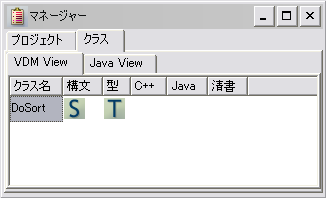
\includegraphics{toolbox}}
\caption{構文および型チェック後の管理画面}\label{fig:toolbox}
\end{center}
\end{figure}

ここで、 \raisebox{-1.0mm}{
\includegraphics[width=0.03\textwidth]{java}}
(\guicmd{Generate Java}) ボタンをクリックすることで、 {\tt DoSort} クラスに対するコード生成を行うことが出来る。
一般的に複数ファイル/クラスの選択が可能で、その場合はそれらすべてが Javaに翻訳される。

図~\ref{fig:interpreter} では、{\tt DoSort} クラスに対してどのように Java コードを生成するかを示している。
見て分かるように、 {\tt  DoSort.java} と呼ばれる Java ファイルがコード生成されている。
これは {\tt DoSort}のJava クラス定義を含むものだ。
 {\tt DoSort.java} ファイルが書き込まれるディレクトリは、プロジェクトファイルが置かれている場所となる。
プロジェクトファイルが存在しない場合は、VDM++ Toolbox の始動ディレクトリにファイルは書き込まれる。

図~\ref{fig:vdmjava} は、 {\tt DoSort}クラスに対するVDM++ 仕様のスケルトンおよび相当するJava生成コードを表す。
生成コードの各部分は、続く章で説明していく。
Appendix \ref{sec:javaDoSort}には、ファイル {\tt DoSort.java} の全体が載せられている。
\begin{figure}[H]
\begin{center}
\mbox{}
\resizebox{9.2cm}{!}{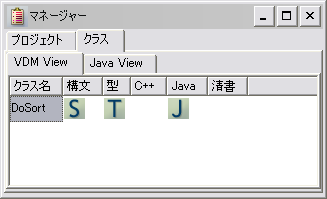
\includegraphics{dosort}}
\caption{{\tt DoSort} クラスをコード生成中}\label{fig:interpreter}
\end{center}
\end{figure}

\begin{figure}
\begin{center}
%\begin{minipage}[t]{2.5in}
\begin{quote}
\begin{small}
\begin{verbatim}
class DoSort

operations
  public Sort: seq of int ==> seq of int
  Sort(l) ==
    ...

functions

  protected DoSorting: seq of int -> seq of int
  DoSorting(l) ==
    ...

  private InsertSorted: int * seq of int -> seq of int
  InsertSorted(i,l) ==
    ...

end DoSort
\end{verbatim}
\end{small}
\end{quote}
%\end{minipage}
VDM++
%\begin{minipage}[t]{2.5in}
%\vspace{2cm}
\begin{quote}
\begin{small}
\begin{verbatim}
public class DoSort {

// ***** VDMTOOLS START Name=vdmComp KEEP=NO
  static UTIL.VDMCompare vdmComp = new UTIL.VDMCompare();
// ***** VDMTOOLS END Name=vdmComp


// ***** VDMTOOLS START Name=Sort KEEP=NO
  public Vector Sort (final Vector l) throws CGException{
    ...
  }
// ***** VDMTOOLS END Name=Sort


// ***** VDMTOOLS START Name=DoSorting KEEP=NO
  protected Vector DoSorting (final Vector l) throws CGException{
    ...
  }
// ***** VDMTOOLS END Name=DoSorting


// ***** VDMTOOLS START Name=InsertSorted KEEP=NO
  private Vector InsertSorted (final Long i, final Vector l)
                              throws CGException {
    ...
  }
// ***** VDMTOOLS END Name=InsertSorted
}
\end{verbatim}
\end{small}
\end{quote}
%\end{minipage}
%Java
\caption{VDM++ と 生成されたJava {\tt DoSort} クラス\label{fig:vdmjava}}
\end{center}
\end{figure}


 \ToolboxName のコマンドライン版からもまた、Javaコード生成は可能である。
 \ToolboxName\ は、コマンド {\tt \vdmde}\index{vdmde!starting}を用いることでコマンドラインから始動される。
Javaコード生成には、 {\tt -j} オプションを用いる。
クラス{\tt DoSort}のコード生成ならば以下のコマンド実行を行う:

\begin{quote}
\begin{verbatim}
vppde -j Sort.rtf
\end{verbatim}
\end{quote}

最初に仕様が構文解析される。
構文エラーが検出されない場合は、仕様に対して可能な限りの適格性のための型チェックがなされることになる。
もし型エラーが検出されなかったならば、最後に、仕様はたくさんの Java ファイルに翻訳される。
記述された仕様に対して、{\tt DoSort} クラス定義を含む {\tt DoSort.java} ファイルが生成される。

注意: もし、仕様がいくつかのクラスを含むか \Tcg\ でコマンドライン版を用いるならば、すべてのクラスは同時にコード生成されている必要がある。

%For each \VDM\ class, one Java file is generated.
%This \path+<ClassName>.java+ file contains the definition of the Java class
%corresponding to the \VDM\ class.

\subsection{生成コードとのインターフェイス}\label{interfacinggettingstarted}

ここまでで、 \VDM\ 仕様からJava コードが生成される地点まで到達した。
これからそのアプリケーションをコンパイルし実行するために、生成された {\tt DoSort} クラスとのインターフェイスをどう記述するかを示す。

\newpage
最初は \VDM{}において、主プログラムを指定することから始める。

\begin{quote}
\begin{verbatim}
01   Main() ==
02     let arr = [23,1,42,31] in
03     ( dcl res : seq of int = [],
04           dos : DoSort := new DoSort();
05       res = dos.Sort(arr);
06     )
\end{verbatim}
\end{quote}

ここで、上記の \VDM\ 仕様と同様の機能性をもったJavaの主プログラムを実装する。
 Java ファイルは主プログラムを含んでいるが、 \JL{} package {\tt jp.co.csk.vdm.toolbox.VDM}の全クラスをインポートすることから始めるべきである:

\begin{quote}
\begin{verbatim}
import jp.co.csk.vdm.toolbox.VDM.*;
\end{verbatim}
\end{quote}

これらのクラスに対して、完全に修飾された名称を記述する必要性が依然のこされる。
\JL{} については、第~\ref{VDMlib}章にさらなる詳細を記述する。
ここでは1つ1つ、上記に挙げたVDM仕様をJavaに翻訳していこう。

行 \path+02+ では整数の並びを指定する。
Javaに翻訳されることで、以下に続くコードを得るであろう:
\begin{quote}
\begin{verbatim}
Vector arr = new Vector();
arr.add(new Integer(23));
arr.add(new Integer(1));
arr.add(new Integer(42));
arr.add(new Integer(31));
\end{verbatim}
\end{quote}


 {\tt Vector} クラスは \texttt{java.util} パッケージに含まれる。
{\tt DoSort}クラスの{\tt Sort}メソッドでは、 {\tt Vector} 型のオブジェクトが入力として要求される。

行 \path+03+ では {\tt seq of int}型の変数 \path+res+ を宣言し、後でソートされた整数列を含めるために用いられる。
これに対応するJava コードは次の通り:

\begin{quote}
\begin{verbatim}
Vector res = new Vector();
\end{verbatim}
\end{quote}

{\tt DoSort}クラスの {\tt Sort} メソッドを呼び出す方法を示そう。
行 \path+04+ では、\path+DoSort+ クラスのインスタンスに対してオブジェクト参照 \path+dos+ を宣言し、行 \path+05+ では、引数としての整数列 \path+arr+ と共に \path+DoSort+ クラスの\path+Sort+ メソッドを呼び出している。
結果は\path+res+に代入される。
Javaに翻訳されることで、以下のコードを得る:

\begin{quote}
\begin{verbatim}
System.out.println("Evaluating Sort("+UTIL.toString(arr)+"):");
DoSort dos = new DoSort();
res = dos.Sort(arr);
System.out.println(UTIL.toString(res));
\end{verbatim}
\end{quote}

\JL{} の一部である {\tt UTIL.toString} メソッドを用いて、  VDM値の ASCII表現を含む列を得る。
このメソッドはここでは、実行中の標準出力に対する関連ログメッセージの印刷に用いられている。

上記に挙げた Java コードは、生成されたJavaコード内メソッドで起こされた例外を取り扱うために、 {\tt try} ブロック内に書かれていなければならない。
 {\tt try} ブロックは {\tt catch clause}に続き、これらの例外を捉えて処理を行う。
生成された Java コードによって起こされる例外はすべて {\tt CGException}クラスのサブクラスであり、これはまた \JL{}の一部である。
このように次の {\tt catch}文が可能である:

\begin{quote}
\begin{verbatim}
try {
...
}
catch (CGException e){
      System.out.println(e.getMessage());
}
\end{verbatim}
\end{quote}

前述の主プログラムは、\path+MainSort.java+ という名のファイルに実装され、これは付録の \ref{sec:main}に全体が載せてある。

\subsection{Javaコードのコンパイルと実行}\label{compileandrun}

主プログラムを手書きすることで、Java コードのコンパイルと実行が可能である。

\cg{} のこの版で生成されたJavaコードは、 Java 開発キット \textbf{1.3}版と相性がよい。

主プログラムは次でコンパイル可能である:
\begin{quote}
\begin{verbatim}
javac MainSort.java
\end{verbatim}
\end{quote}

 {\tt CLASSPATH} 環境変数が \JL{}すなわち {\tt VDM.jar} ファイルを含めていることを確認しよう。
 もしUnix Bourne シェル または 互換性のあるシェルを用いているのであれば、これは以下のコマンドで行うことができる:

\begin{quote}
\begin{verbatim}
CLASSPATH=VDM_Java_Library/VDM.jar:$CLASSPATH
export CLASSPATH
\end{verbatim}
\end{quote}%$

 \JL{} がインストールされたディレクトリ名称を {\tt VDM\_Java\_Library} と置き換えよう。

もし Windowsベースのシステムを使用しているのであれば、 \texttt{CLASSPATH}環境変数は \texttt{autoexec.bat} において、あるいはコントロールパネルの \texttt{System} アイコンから、更新できる。
 Windowsに対しては、区切り文字は ``{\tt :}'' ではなく ``{\tt ;}'' を用いなければならないことに注意しよう。

主プログラム \path+MainSort+ は、これで実行可能である。
この出力を以下に載せる。
\begin{quote}
\begin{verbatim}
$  java MainSort
Evaluating Sort([23, 1, 42, 31]):
[1, 23, 31, 42]
$
\end{verbatim}
\end{quote}

この章では、どのように \tcg を使用するかについて、簡単な導入を示した。
以下の章ではもう少し詳細に \tcg\ の様々な局面を記述する。
以降は、生成コード部分の提示は常に、論点に関連する部分のみのテキスト提示とするので注意しよう。

\newpage
\section{コードジェネレータ − 発展事項}
\label{advancedissues}

第~\ref{invoking}章では \tcg{} への簡単な導入を示した。
この章は、以下に続く質問への答えを与えることになる:

\begin{itemize}
\item VDM++仕様からJavaコードを生成するときに、どのようなオプションを使用できるか? (第~\ref{options}章)
\item 仕様が暗黙または予備的な関数/操作を含める場合には、何が行えるか? (第~\ref{implicit}章)
\item 生成されたJavaコードを手書きコードと置き換える可能性は? (第~\ref{substituting}章)
\item  \VDM\ 仕様がコンパイル可能な正しいJavaコードに翻訳されるために満たすべき要件は何か?
(第~\ref{sec:unsupported}章)
\end{itemize}

\subsection{VDM++ to Java コードジェネレータのオプション}
\label{options}

VDM++ 仕様からJavaコードを生成するとき、生成コードに影響を与える1つ以上の次のオプションを選択することができる。
利用可能なオプションを見るために、図~\ref{fig:optionsmenu}に示すように、オプションメニューから \textit{Java Code Generator} エントリーを選択しよう。

\begin{figure}[H]
\begin{center}
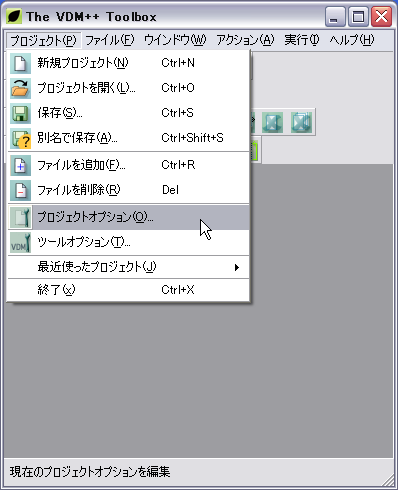
\includegraphics[width=.8\textwidth]{optionsmenu}
\caption{Java コードジェネレータのオプションの選択}\label{fig:optionsmenu}
\end{center}
\end{figure}

図~\ref{fig:options}に示されるように、 \tcg\ において様々なオプションが利用可能である。
\begin{figure}
\begin{center}
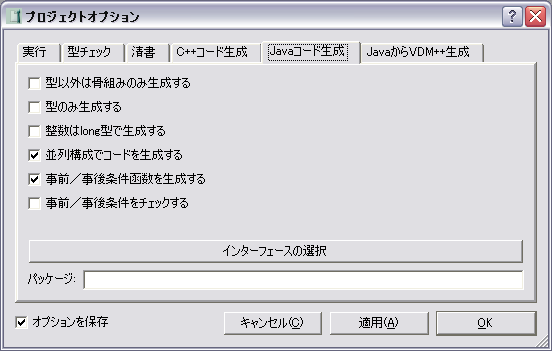
\includegraphics[width=.8\textwidth]{options}
\caption{Java コード生成のためのオプション}\label{fig:options}
\end{center}
\end{figure}
これら各オプションは以下に記述している。
これらオプションすべてが、 \tcg のコマンドライン版でも利用可能であることに注意しよう。
以下の各オプション名称の後の括弧内に、適切なフラグを提示している。
既定の動作もまた、既定で与えられたオプションで指定された動作が用いられないという意味の ``off'' や、動作が用いられるという意味の ``on'' に記載されている。

\begin{description}
\item [ ({\tt -s})型以外に対してスケルトンのみのコード生成]
  スケルトンクラスを生成するために、このオプションを指定する。
スケルトンクラスはすべての型、値、インスタンス変数定義を含むが、空の関数や操作の定義は含まないクラスである。
既定: \textbf{off}
%\item [Code generate small types]
%  The default behaviour of the Code Generator is to
%  generate code with ``big'' types, i.e.\ the wrapper classes {\tt
%  Integer}, {\tt Double}, {\tt Boolean} and {\tt Character} are used
%  in the generated code. Specify the {\tt -m} option in order to
%  generate code using the ``small'' types   {\tt int}, {\tt double},
%  {\tt boolean} and {\tt char}. Note, that ``small'' types are only
%  used in type definitions and method headers. Therfore, this option
%  implies the {\tt -s} option, because otherwise the generated code
%  would not be compilable. It is not possible to insert primitive
%  data types in compound data types such as sets and sequences. %{\tt -m}
\item [Code generate only types ({\tt -u}) 型のみをコード生成 ({\tt -u})]
  VDM++ 型定義に対してJavaコードを生成したいというだけのとき、このオプションを指定する (つまり 関数、操作、インスタンス変数、値、は生成されない)。既定: \textbf{off}.%
\item [Longs (\texttt{-L})として整数をコード生成]
  このオプションを使用することで、VDM++ 整数値と変数をJavaの\texttt{Integer}ではなく \texttt{Long}として生成が可能である。
既定: \textbf{off}
\item [並列構成要素に伴うコードのコード生成(\texttt{-e})]
  このオプションは、コードジェネレータが並列支援を含めるコード生成を行うことを強要するために用いられる。
この詳細は第~\ref{concmain}章を参照のこと。
既定: \textbf{on}.
\item [事前事後の関数/操作のコード生成 (\texttt{-k})]
事前事後条件に対するJavaメソッドやそれらの不変数をコード生成するために、 このオプションを指定する。
既定: \textbf{on}%{\tt -k}
\item [事前および事後条件のチェック (\texttt{-P})]
 このオプションを、関数の事前事後条件のインラインチェック生成のために指定する。
チェックが失敗した場合に例外を発生する。
この意味は、事前事後条件としての前述のオプションが、コンパイル可能なコードのために生成されるべきであることを含めている。
既定: \textbf{off}.%{\tt -P}
\item [パッケージ (\texttt{-z}) \textit{packagename}]
  コードジェネレータの既定の動作は、ディレクトリ内に生成されたJavaファイルを書き出すことであり、このディレクトリとはプロジェクトファイルが置かれている場所か、あるいはプロジェクトファイルが存在しない場合は \ToolboxName\ がスタートした場所である。
ファイルは名称のない既定パッケージの一部である。
生成されたJavaクラスを含むはずの指定パッケージを生成するために、このオプションを指定する。
コードジェネレータは、生成ファイルを含めるため与えられたパッケージ名称を使った新しいディレクトリを作成し、生成ファイルには適切な  \texttt{package} 文が含まれることになる。%{\tt -z package\_name}
\item [インターフェイスの選択 (\texttt{-U})]
  Javaインターフェイスとして生成されるべきクラスを選択する。詳細は第~\ref{sec:interfaces}章を参照。
\end{description}

コマンドラインから \ToolboxName\ をスタートさせる場合、以下のコマンドが用いられる必要がある:

\begin{quote}
\begin{verbatim}
vppde -j [options] specfile(s)
\end{verbatim}
\end{quote}


\subsection{暗黙のかつ予備的な関数/操作の実装}\label{implicit}

暗黙の関数/操作および予備的な関数/操作(``{\tt is not yet specified}''で指定されたもの) が、 \tcg{}によっても同じ方法で取り扱える。
予備的な操作定義を含む以下の VDM++ クラス定義を見よう。

\begin{quote}
\begin{verbatim}
class A
operations
op:() ==> int
op() == is not yet specified;
end A
\end{verbatim}
\end{quote}

このクラスは以下のように生成されることになる:

\begin{quote}
\begin{verbatim}
public class A {
  protected external_A child = new external_A(this);
  private Integer op () throws CGException{
    return child.impl_op();
  }
};
\end{verbatim}
\end{quote}

上述のコードから見てとれるように、クラス \texttt{A}A は型{\tt external\_A}の保護されたインスタンス変数 {\tt child} を含める。
これは、暗黙の関数/操作または予備的な (``{\tt is not yet   specified}''で指定された)関数/操作を含めるすべてのクラスに当てはまる。
クラスがこれらの定義をいくつか含めるとしても、その外部クラスは1つのインスタンスしか存在しないはずである。

 \path+op+ メソッドは、このインスタンスの \path+impl_op+ という名のメソッドを呼び出すことになる。\footnote{{\tt impl} は ``Javaで実装されるべき''ことを表す。}  \path+impl_op+ メソッドの結果は \path+op+ メソッドの結果として返される。

したがってクラス {\tt external\_A}にメソッド\path+impl_op+ を実装することは、ユーザーの責任である。
メソッド \path+impl_op+の入出力パラメータは、メソッド \path+op+のそれと同じでなければならない。

もし VDM++ クラスが1つ以上の暗黙の関数/操作または予備的な関数/操作(``{\tt is not yet specified}''で指定されたもの)を含むとすれば、すべてのメソッドが\path+external_<CLASSNAME>+に実装されていなければならない。

ユーザーの外部クラスファイルをユーザーが実装するのを容易とするために、 \tcg\ はこれに対する \texttt{external\_A.java} ファイルを生成する。
このファイルの支援で、生成された Java コードはコンパイル可能となる。
しかしながら予備的な関数が呼ばれた場合は、実行時エラーが起きることになる。
{\tt external\_A}クラスを含む{\tt external\_A.java} ファイルは、以下におかれている。

\begin{quote}
\begin{verbatim}
public class external_A {
  A parent = null;
  public external_A (A parentA) {
    parent = parentA;
  }
  public Integer impl_op () throws CGException{
    UTIL.RunTime("Preliminary Operation op has been called");
    return new Integer(0);
  }
};
\end{verbatim}
\end{quote}

 {\tt external\_A} クラスを実装するための最も簡単な方法は、テンプレートクラスを修正すること、つまりユーザーは次のコードに対して、ユーザー定義コードに生成コードを置き換えることが可能な通常の方法で、置き換えを行う必要がある。

\begin{quote}
\begin{verbatim}
UTIL.RunTime("Preliminary Operation op has been called");
return new Integer(0);
\end{verbatim}
\end{quote}

(詳細は第~\ref{substituting} 章を参照)


%Once the user has tailored the {\tt external\_<ClassName>.java} file,
%it has to be insured, that a new code generation does not overwrite
%it with a new file. Therefore, when an {\tt
%external\_<ClassName>.java} already exists, an {\tt
%external\_<ClassName>.java.default} file is generated instead.

注意したいのは、外部クラスに対して生成されたコンストラクタが、入力パラメータとしてクラス {\tt A} のインスタンスを取り入れ変数 {\tt parent}に代入することである。
この方法で、予備的な操作定義の実装はクラス {\tt A}のパブリック状態にアクセス可能である。
クラスの内部状態に作用することが許されないため、予備的な関数に対応するJavaメソッドがこのコンストラクタを用いることになる。
しかしそれらはある操作を呼び出すことで、間接的に内部状態に作用が可能となる。

暗黙的に定義された関数と操作は、 ``{\tt is not yet specified}''節を含む予備的な関数や操作の仕様と同じ方法で取り扱われる。

注意したいのは、外部クラスが暗黙および予備的な操作と関数を含めることが可能であることだ。
生成された定型書式では、生成された次のような実行時エラーメッセージで区別可能である:

\begin{quote}
\begin{verbatim}
UTIL.RunTime("Preliminary Operation op has been called");
\end{verbatim}
\end{quote}

これは {\tt op} という名の予備的な操作定義に対するものであり

\begin{quote}
\begin{verbatim}
UTIL.RunTime("Implicit Function f has been called");
\end{verbatim}
\end{quote}

これは {\tt f}という名の暗黙の関数定義に対するものある。

\subsection{抽象クラスの生成}

VDM++ クラスは、予備的な関数あるいは操作の定義を含むかあるいは抽象クラスのサブクラスであるならば 抽象なものであり、継承されている抽象の関数や操作に対しての実装は提供しないものとなる。
このように抽象であることは、 VDM++ クラスの間接特性である。

一方で、Java は抽象クラスの基本概念を提供している。
したがって、Java コードを生成するときに抽象と識別される VDM++ クラスは、抽象Javaクラスとして生成されることになる。
たとえば、 以下のVDM++ クラス \texttt{A}、\texttt{B} 、\texttt{C} を考察してみよう:

\begin{quote}
\begin{verbatim}
class A

instance variables
  protected m : nat := 1

operations
  public op : nat ==> nat
  op(n) == is subclass responsibility;

functions
  public f : int -> int
  f(i) == is subclass responsibility

end A

class B is subclass of A

operations
  public op : nat ==> nat
  op(n) ==
    return m + n

end B

class C is subclass of B

functions
  public f : int -> int
  f(i) == i + 1

end C
\end{verbatim}
\end{quote}
クラス \texttt{A} は予備的関数や操作を含み、そのため抽象である。
したがって次のようなコード生成がなされる:
\begin{quote}
\begin{verbatim}
public abstract class A {

  protected Integer m = null;
  public abstract Integer op (final Integer n) throws CGException;
  public abstract Integer f (final Integer i) throws CGException;

}
\end{verbatim}
\end{quote}
クラス \texttt{B} は抽象クラス \texttt{A}を継承し、関数 \texttt{f}の実装を提供していない。
したがって抽象でもある:

\begin{quote}
\begin{verbatim}
public abstract class B extends A {

  public Integer op (final Integer n) throws CGException {
    return new Integer(m.intValue() + n.intValue());
  }
}
\end{verbatim}
\end{quote}

最後は、クラス \texttt{C} は \texttt{B} から継承し \texttt{f}の実装を提供するためにある。
したがって通常クラスである:
\begin{quote}
\begin{verbatim}
public class C extends B {

  public Integer f (final Integer i) throws CGException{
    return new Integer(i.intValue() + new Integer(1).intValue());
  }
}
\end{verbatim}
\end{quote}


\subsection{生成された Java コード部分の置き換え}\label{substituting}

標準的な応用として、生成コードに対し、例えば外部ライブラリや手書きコードといった他コードと相互作用を行う必要が生じてくるだろう。
このような相互作用を手助けするため、生成コードの修正が可能で、しかも \tcg\ が再実行されてもそれらの修正が上書きされない方法で、可能である。

これは、 \textit{キープタグ}の使用を通して達成される。
これらは生成されたJavaコードにおいてはコメントであるが、 そのコードの比率が上書されるべきか否かを \tcg\ が決定するときに用いるものである。

たとえば以下の例題を考えよう:
\begin{quote}
\begin{verbatim}
class Date

types
  public Day = <Mon> | <Tue> | <Wed> | <Thu> | <Fri> | <Sat> | <Sun>;
  public Month = <Jan> | <Feb> | <Mar> | <Apr> | <May> | <Jun>
        | <Jul> | <Aug> | <Sep> | <Oct> | <Nov> | <Dec>;
  public Year = nat

instance variables
  d : Day;
  m : Month;
  y : Year

operations

  public SetDate : Day * Month * Year ==> ()
  SetDate(nd,nm,ny) ==
  ( d := nd;
    m := nm;
    y := ny );

  public today : () ==> Date
  today() ==
    return new Date()
end Date
\end{verbatim}
\end{quote}
 VDM++ も \ToolboxName\ も時間の基本概念を持たないため、\texttt{today}に完璧な仕様を与えることはできない。
生成コードで \texttt{today} は次のようになる:
\begin{quote}
\begin{verbatim}
// ***** VDMTOOLS START Name=today KEEP=NO
  public Date today () throws CGException{
    return (Date) new Date();
  }
// ***** VDMTOOLS END Name=today
\end{verbatim}
\end{quote}
関数定義の上下のコメントは、この関数に対するキープタグに相当する。
キープタグでは以下の情報が得られる:
\begin{itemize}
\item タグが適用される実体の名称 (実体を構成するものは次で述べられる)。
 テキスト\texttt{Name=}の直後に置かれる。
\item この実体が保存されるべきか上書きされるべきかを示すフラグ。
 \texttt{KEEP=}の後にテキストで与えられる。
もし\texttt{NO}ならば実体は上書きされる; \texttt{YES}ならば保存される。
ファイル生成時の既定は \texttt{NO}。
\end{itemize}
現在の日付を実際通りに戻すように、この関数を修正したいと仮定する。
これは、 Java 開発キットの一部として提供されている \texttt{Calendar} クラスを用いて可能である。
\begin{quote}
\begin{verbatim}
// ***** VDMTOOLS START Name=today KEEP=YES
  public Date today () throws CGException{
    Calendar c = Calendar.getInstance();
    Date result = new Date();
    Object td = new Object(), tm = new Object();
    switch (c.get(Calendar.DAY_OF_WEEK)){
    case Calendar.MONDAY:
        td = new quotes.Mon();
        break;
    ...
    }
    switch (c.get(Calendar.MONTH)){
    case Calendar.JANUARY:
        tm = new quotes.Jan();
        break;
    ...
    }
    result.SetDate(td, tm, new Integer(c.get(Calendar.YEAR)));
    return result;
  }
// ***** VDMTOOLS END Name=today
\end{verbatim}
\end{quote}
最初にキープタグが \texttt{YES}に変化してしまっていることに注意しよう。
これは変更が保存されたことを保証している。
関数本体はしたがって通常のJava コードであり、任意の外部クラスで用いることができる。

現存の実体の変更に加えて、 Java ファイルに新しい実体の追加ができる。
既定の\texttt{toString} メソッド ( \texttt{java.lang.Object}から継承)を日付に適用したものに置き換えたいと仮定しよう。
以下をクラス定義に追加できるだろう。
\begin{quote}
\begin{verbatim}
// ***** VDMTOOLS START Name=toString KEEP=YES
  public String toString(){
      return d.toString() + m.toString() + y.toString();
  }
// ***** VDMTOOLS END Name=toString
\end{verbatim}
\end{quote}

\subsubsection{実体}

キープタグを用いて保存できた生成 Java ファイルにおいて、実体は1つの領域である。
これは以下の1つとなる可能性がある:
\begin{itemize}
\item トップレベルのクラス要素変数。
\item トップレベルのクラスメソッド(コンストラクタを含める)。
\item 内部クラス。
\item インポート宣言の集まり。
\item パッケージ宣言。
\item ヘッダーコメント つまりファイルの先頭領域には、たとえばバージョン管理情報といったコメントを置くことができる。
\end{itemize}
キープタグは、インターフェイスとして生成されたクラスと共に用いられることもあることは注意しよう (第~\ref{sec:interfaces}章参照); この場合も同じ規則が適用され、クラスの代わりにインターフェイスが読み込まれる。

事前に定義された3つのタグ名称: ヘッダーコメントのための\texttt{HeaderComment}、パッケージ宣言のための\texttt{package} 、インポート宣言のための \texttt{imports} 、は生成されたファイル中でよく現れる。

\subsubsection{キープタグのための規則}

キープタグを使用するときは以下の規則に従わなくてはならない。
\begin{itemize}
\item 各タグ名称は唯一のものでなければならない。
\item タグは同一レベルでなければならない、つまりタグのネストは不可能である。
\item クラス定義の外部のみで現れる可能性のあるタグは、\texttt{HeaderComment}、 \texttt{package} 、 \texttt{imports}である。
\item 付加された実体はクラス定義の \textbf{内部に} 、それも先頭部分に現れなければならない。このように、たとえばある関数がクラス内部に追加された場合、クラス内部全体が\texttt{YES}とタグづけされなければならない。
\item タグ保持の構文では、case文と空白は細心の注意を払うべきである。正確に後ろを続けていく必要がある。
\end{itemize}
これらの規則に従わないとき、コードは上書きされてしまう可能性がある。
しかしながら元のファイルは常にバックアップされるため、これが必ずしも致命的となることはない


\subsection{インターフェイスの生成}\label{sec:interfaces}

\Tcg\ は Java インターフェイス \cite{Gosling&00}の生成を可能としている。
 \VDM\ クラスは以下の条件に適応する場合は、インターフェイスとして生成される可能性がある:
\begin{itemize}
\item このクラスで定義された関数と操作のすべてが、本体 \texttt{is subclass responsibility}を含む。
\item インスタンス変数を含まないクラスが、このクラス中に定義されている。
\item このクラスで定義されたすべての型が、パブリックである。
\item このクラスで定義されたすべての値は、直接の定義が可能である (直接定義される値の意味の説明は第~\ref{values}章を参照)。
\item このクラスのすべてのスーパークラスはインターフェイスとして生成可能である。
\end{itemize}
たとえば、図~\ref{fig:interfacesex}の例題を考えてみよう。
\begin{figure}
\begin{quote}
\verbatiminput{manexamples/interfaces.vpp}
\end{quote}
\caption{インターフェイス例題}\label{fig:interfacesex}
\end{figure}
クラス \texttt{A} は明らかにインターフェイスとして生成されるための要件を満たすが、なぜなら直接定義された値をもち、その関数と操作すべてが \texttt{is subclass responsibility}だからである。
クラス \texttt{B} もまたインターフェイスとして生成可能だが、なぜなら抽象関数1つだけが与えられ、インターフェイスとして生成が可能なクラスから継承しているからである。
しかしクラス \texttt{C}はインターフェイスとして生成はできない、なぜなら抽象でない関数の宣言を行っているからである。

どのクラスをインターフェイスとして生成するべきかの選択には、オプションダイアログボックス(第~\ref{options}章に記述されている) の \textit{インターフェイス選択} ボタンをクリックしよう。
 図~\ref{fig:interfaces1}で示すように、新しいダイアログボックスが開く。

\begin{figure}
\begin{center}
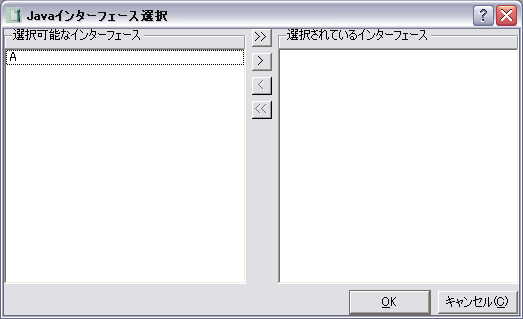
\includegraphics[width=.8\textwidth]{interfaces1}
\end{center}
\caption{初期インターフェイス選択ダイアログ}\label{fig:interfaces1}
\end{figure}

最初は、インターフェイス -\texttt{A}としては唯1つクラスが生成される可能性がある。
これが選択されると ( \textit{追加}ボタンをクリックすることにより)、 図~\ref{fig:interfaces2}に示されるようにダイアログは更新される。

\begin{figure}
\begin{center}
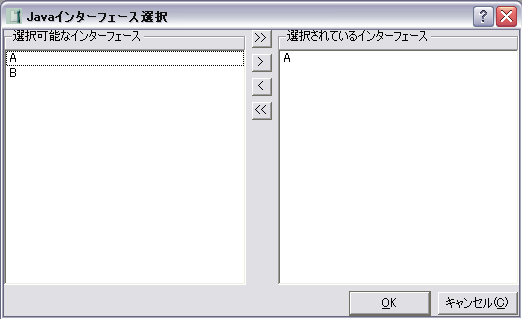
\includegraphics[width=.8\textwidth]{interfaces2}
\end{center}
\caption{更新されたインターフェイス選択ダイアログ}\label{fig:interfaces2}
\end{figure}

ここで可能なインターフェイスの一覧に \texttt{B} が現れていることに注目しよう。
もしこのスーパークラス - \texttt{A} - がインターフェイスであるならば、これはインターフェイスとして生成されることのみ可能となるためである。
選択インターフェイスの一覧から \texttt{A} が今取り除かれたら、\texttt{B}は自動的に一覧から取り除かれるが、その時点でもはやインターフェイスの基準を満たさないからである。

インターフェイスとして生成されるべきクラスが選択されると、コード生成は通常通りに開始する。
\texttt{A}に対して以下のコードが生成されるはずである:
\begin{quote}
\begin{verbatim}
public interface A {

// ***** VDMTOOLS START Name=v KEEP=NO
  private static final Integer v = new Integer(1);
// ***** VDMTOOLS END Name=v


// ***** VDMTOOLS START Name=op KEEP=NO
  public abstract Integer op (final Integer n) throws CGException;
// ***** VDMTOOLS END Name=op


// ***** VDMTOOLS START Name=f KEEP=NO
  public abstract Integer f (final Integer n) throws CGException;
// ***** VDMTOOLS END Name=f

}
\end{verbatim}
\end{quote}

Toolboxのコマンドライン版を用いてもまたインターフェイスの選択は可能であり、この場合 \texttt{-U} オプションを用いる:
\begin{quote}
\begin{alltt}
vppde -j -U \textit{class\{,class\}} specfiles
\end{alltt}
\end{quote}
もしクラスが上記のインターフェイス基準を満足させないとする場合、以下のエラーメッセージが生成されるだろう:
\begin{quote}
\begin{alltt}
Can not generate class \textit{class} as an interface - ignored
\end{alltt}
\end{quote}



\subsection{制限}\label{sec:unsupported}

すべての \VDM\ 仕様でJavaコード生成が可能というわけではない。
コンパイル可能で正しいJavaコードに翻訳されるために、 \VDM\ 仕様はある要件を満たす必要がある。
これらの制限は主に2つの理由が原因で引き起こされる:
\begin{itemize}
\item 用いられる翻訳アルゴリズムの制限: \VDM\ および Java は2つの異なる言語であること。
わずかな例として、 \VDM\ 構成要素の何らかの翻訳が正しくないJavaコードを導く可能性がある。
このことから引き起こされる制限は、第~\ref{lim1}章に並べている。
並べた要件を満たさない\VDM\ 仕様は、コンパイル可能でない誤ったJavaコードを導く可能性がある。
 Javaへ翻訳できない \VDM\ 特性にぶつかると、 \Tcg\ は警告/エラーのメッセージを生成する。
\item 翻訳の範囲制限:
コードジェネレータはすべての構成要素をサポートしているわけではない。
第~\ref{lim2}章では、 \tcg{}でサポートされない \VDM\ 構成要素をまとめている。
これらの構成要素はコンパイルできないJavaコードではないが、これらに対して生成されたコードを実行すると実行時エラーとなる。
\Tcg\ はサポートされていない構成要素に出会えば必ず、警告を与えることになる。
\end{itemize}
Java と VDM++ の意味論においては、プライベートメソッドが動的配置に伴ってどう扱われるかが異なることに注意しよう。
以下の例題を考える:

\begin{minipage}{.55\textwidth}
\begin{quote}
\begin{verbatim}
class C
operations
public op1 : () ==> seq of char
op1() == op2();

private op2 : () ==> seq of char
op2() == return "C`op2"
end C
\end{verbatim}
\end{quote}
\end{minipage}
\begin{minipage}{.45\textwidth}
%\begin{quote}
\begin{verbatim}
class D is subclass of C
operations
public op3 : () ==> seq of char
op3() == op1();

private op2 : () ==> seq of char
op2() == return "D`op2"
end D
\end{verbatim}
%\end{quote}
\end{minipage}

 Javaにおいて、式 \texttt{new D().op3()} は結果\texttt{C`op2}をもたらす。
 \VDM\ においては、同じ式が \texttt{"D`op2"}をもたらす。

\subsubsection{言語の違いに起因する \VDM\ 仕様の要件}
\label{lim1}

 \VDM\ 仕様は、 {\em コンパイル可能} で {\em 正しい} Java コードを生成するために、以下の要件を満たさなければならない:

\begin{itemize}
\item ``{\em 型情報不明}''という型チェッカー警告は取り除かれるべきであるが、生成コードでエラーに導くことが可能であるからである。
もしVDM 構成要素に型情報が失われていたら、\Tcg\ は正しいJava型の生成ができない。

節、インスタンス変数、型、値、関数、操作は同じ名称をもつことはない。
さらには、名称の再宣言は避けるべきである。
この意味は、たとえば以下の \VDM\ 仕様は変数名称 {\tt a} が再宣言されているため、コンパイル不可能な結果となるだろう、ということである:

\begin{quote}
\begin{small}
\begin{verbatim}
f : int | (int * int) ==> bool
f(a) ==
  cases a:
    2 -> return true,
    mk_(a,b) ->  return false,
    others -> let a = 1 in return true
  end;
\end{verbatim}
\end{small}
\end{quote}

抽象の操作/関数は、それらを実装する操作/関数と同じ型をもつ必要がある。
以下の例題を考えよう:
\begin{quote}
\begin{small}
\begin{verbatim}
class A
operations
  m: nat ==> nat
  m(n) == is not yet specified;
end A

class B is subclass of A
operations
  m: nat ==> nat
  m(n) = return n+n;
end B
\end{verbatim}
\end{small}
\end{quote}
もし\texttt{B`m} の型が\texttt{A`m}の型とぴったりとは一致しない場合、\texttt{A`m} はまだ \texttt{B}では抽象であり、したがって \texttt{B}は抽象クラスということになる。

\item 多重継承のため制限形式が用いられる可能性がある。
しかし、これに含まれるクラスは第~\ref{sec:interfaces}章に記載された条件を満たしている必要がある。

case文のすべての場合わけがreturn文を含めるならば、case文は {\tt others} 岐をもたなくてはならない。
そうでない場合には、生成されたJavaコードをコンパイルしながら Java コンパイラは ``{\em Return required}'' エラーを生成する。
\item 不要なコードは避けるべきである。
以下の例題を考えよう:

\begin{quote}
\begin{small}
\begin{verbatim}
operations
  m : nat ==> nat
  m(n) ==
    (return n;
     a:= 4;
    );
\end{verbatim}
\end{small}
\end{quote}

文 {\tt a:= 4;} は決して実行されることはなく、生成されたJavaコードをコンパイルしながら ``{\em Statement not reached}'' エラーに導く。
\item スーパークラスにおける操作呼出しが名称で修飾された場合、生成コードは誤ったものとなる可能性がある。
以下の例題を見よう:

\begin{quote}
\begin{small}
\begin{verbatim}
class A

operations

public SetVal : nat ==> ()
SetVal(n) == ...;

end A

class B is subclass of A

operations

public SetVal : nat ==> ()
SetVal(n) == ...

end B

class C is subclass of B

operations

public Test : () ==> ()
Test() ==
  ( self.SetVal(1);
    self.B`SetVal(1);
    self.A`SetVal(2)
  )

end C

class D

instance variables
  b : B := new B()

operations

public Test: () ==> ()
Test() ==
  (b.SetVal(1);
   b.B`SetVal(5);
   b.A`SetVal(2)
  )

end D
\end{verbatim}
\end{small}
\end{quote}

まずはクラス {\tt C}から見よう:
文 {\tt self.SetVal(1)}はクラス {\tt C}における {\tt SetVal} 操作を呼び出し、Javaにおいて {\tt this.SetVal(1)} としてコード生成されることになる。
文 {\tt self.B`SetVal(1)}はクラス {\tt B}における{\tt SetVal}操作を呼び出し、Javaにおいて {\tt super.SetVal(1)} としてコード生成されることになる。
 Java では、クラス{\tt A}の {\tt SetVal()} メソッド呼び出しは不可能である。
文 {\tt self.A`SetVal(2)} は {\tt super.SetVal(2)}としてコード生成されるだろう。
クラス {\tt B}に {\tt SetVal} 操作がなかったなら、これは正しくなるはずである。
しかし上記の場合、これは VDM++ 仕様に適合しない。
 2つの操作呼び出し {\tt self.B`SetVal(1)} と {\tt self.A`SetVal(2)} はコードジェネレータに警告 ``{\em Quoted method call is code generated as a call to super}''を与える原因となる。
ユーザーはしたがって正しいメソッドが呼び出されたかの確認ができる。

  次にクラス {\tt D}を見よう:
文 {\tt b.SetVal(1)} はクラス {\tt B}の {\tt SetVal} 操作を呼び出し、Javaで {\tt b.SetVal(1)} としてコード生成されることになる。
Javaではオーバーライドしているクラスの外部からオーバーライドされたメソッドを起動することはできない。
 したがってクラス {\tt A}で {\tt SetVal}メソッドを呼び出す方法はない。
クラス {\tt D}で引用された操作呼び出しは、したがってすべて {\tt b.SetVal(1)}としてコード生成される。
しかしながらコード生成は、ユーザーに知らせるために警告 ``{\em Quoted method call is removed}'' を発するはずである。

\item Javaにおける整数型およびダブル型に対する最大 (最小)値は、 \VDM{}のそれぞれの値より小さい(大きい)。
Javaでは有効でない値が、生成されたJavaコードの実行時にエラーに導く。
\end{itemize}

\subsubsection{サポートされていない構成要素}
\label{lim2}

 \tcg\ のこの版では、以下の \VDM\ 構成要素はサポートされていない:

\begin{itemize}

%% Is not part of the language manual any longer!
%\item The Real-time part of \VDM{}.
\item 式:

  \begin{itemize}
  \item ラムダ式
  \item 関数に対する合成、繰り返し、同等
  \item 型判定式
#ifdef VICEMAN
  \item time式
#endif VICEMAN
  \item 高次関数。
  \item ローカル関数定義。
  \item 関数型インスタンス化式。しかし、以下の例題の中にあるように、コードジェネレータが適用式と組み合わさることで関数型インスタンス化式をサポートする:

\begin{quote}
\begin{verbatim}
Test:() -> set of int
Test() ==
  ElemToSet[int](-1);

ElemToSet[@elem]: @elem +> set of @elem
ElemToSet(e) ==
  {e}
\end{verbatim}
\end{quote}

  \end{itemize}

\item 文:
  \begin{itemize}
  \item 仕様記述文
#ifdef VDMSL
  \item call文内の `{\sf using}'
#endif VDMSL
#ifdef VDMPP
  \item startlist文
#endif VDMPP
#ifdef VICEMAN
  \item duration文とcycles文は無視される
#endif VICEMAN
  \end{itemize}

\item 型束縛 (\langmancite 参照)ただし次の中:

  \begin{itemize}
  \item Let-be-st 式/文
  \item 列、集合、写像の包括式
  \item Iota式 と修飾式
  \end{itemize}

例題として、以下の式が\tcg によりサポートされている:

\begin{quote}
\begin{verbatim}
let x in set numbers in x
\end{verbatim}
\end{quote}

一方で以下はサポートされていない (型束縛 \verb+n: nat+に起因する):

\begin{quote}
\begin{verbatim}
let x: nat in x
\end{verbatim}
\end{quote}

\item パターン:

  \begin{itemize}
  \item 集合結合パターン。
  \item 列連結パターン。
  \end{itemize}

#ifdef VDMSL
\item Local Function Definitions.

\item Higher order function definitions.

\item Function Values.

\item Parameterized modules.
#endif VDMSL
\end{itemize}

#ifdef VICEMAN
CPUとBUSesへのシステム仕様と対応する展開は無視されます。
Javaコードがそのようなシステム記述から生成されると、生成コードは、役に立たなく、コンパイルできないでしょう。
同様に、操作定義の \keyw{async} キーワードは無視されます。
#endif VICEMAN

\Tcg\ はこれらの構成要素を含む仕様に対してコンパイル可能なコードを生成できるが、サポートされていない構成要素を含む分岐が実行された場合は、コードの実行は実行時エラーという結果となる。
以下の関数定義を考えよう:

\begin{quote}
\begin{verbatim}
f: nat -> nat
f(x) ==
  if x <> 2 then
    x
  else
    iota x : nat & x ** 2 = 4
\end{verbatim}
\end{quote}

\path+f+ に対して生成されたコードは、コンパイルされることになる。
しかし \path+f+ に相当するコンパイルされた Java コードは、  \path+f+ に値2が適用されれば、iota式の型束縛はサポートされず実行時エラーという結果に終わるだろう。

注意したいのは、 \Tcg\ はサポートされていない構成要素に出会った場合は必ず警告を与えるはずだということである。
上記の関数{\tt f} に対するコード生成が、図~\ref{fig:cg_error}で示される {\em Error} ウィンドウに導く。

\begin{figure}[H]
\begin{center}
\mbox{}
\resizebox{9.2cm}{!}{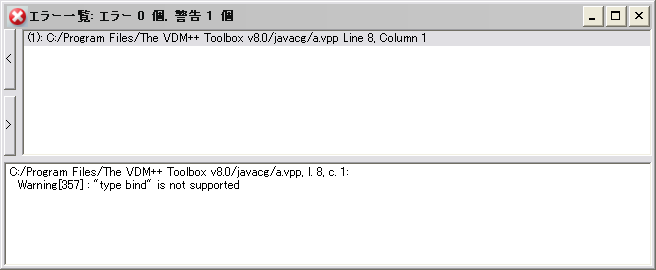
\includegraphics{warning}}
\caption{コードジェネレータにより生成された警告}\label{fig:cg_error}
\end{center}
\end{figure}

\newpage
\section{\VDM\ 仕様のコード生成}
\label{sec:relation}

この章では、 \VDM\ 構成要素がコード生成される方法を詳細に記述していく。
この記述は、\tcg\ を専門的に利用しようとする場合には集中して学習すべき内容である。
始めは \JL{}への導入を行うが、これが \VDM\ 仕様コード生成の基礎を形成する。
その後、上記で述べた \VDM\ 構成要素1つ1つに対して生成されるコードを述べていく。

\subsection{VDM Java ライブラリ}
\label{VDMlib}

生成コードのデータ改編は、 \JL{}に基づき、パッケージ {\tt jp.co.csk.vdm.toolbox.VDM}に実装されている。
ここでは、このライブラリに短い導入を与えるだけとする。
さらには、 {\em javadoc} プログラムにより生成されたHTML文書で説明されている。
このライブラリの全体理解のためには、説明書を読むべきである。
 {\em javadoc} プログラムを使用した HTML 文書生成方法についての記述は、付録~\ref{install}を参照のこと。

 \JL{} は以下の\VDM\ データ型の固定実装を提供する:

\begin{itemize}
%\item Sequence Type
%\item Set Type
%\item Map Type
%\item Quote Type
%\item Token Type
\item Product/Tuple Type
\item 積型/組型
%\item Optional Type
\item Record Type
\item レコード型
\end{itemize}

これらの型のそれぞれに対して、1つのクラスが、相当するVDM++ 型と同じパブリックメソッドを提供しながら実装されてくる。
これらクラスは Java 言語により提供されたクラスの先頭に実装される。

\VDM\ データ型で上記で並べていないもの(基本 \VDM\ データ型、集合型、列型、写像型、\path+Optional+型、\path+Object Reference+型)は、Java言語自身の一部であるクラス/構成要素 かあるいは標準Java開発キット(JDK)の一部配布により表現される。

上記に挙げた \VDM\ データ型の実装の提供に加えて、 \JL{} はさらに2つのクラスを提供する:

\begin{itemize}
\item このクラスは補助メソッドを含むが、これは生成されたコードに用いられ、またユーザーが生成コードとインターフェイスをとるときに使用できる。
これらの補助的メソッドのうちもっとも重要なものを以下に並べる:
\begin{itemize}
\item {\tt clone}: VDM 値を (綿密に) 模倣する。
しかしながら、\VDM\ クラスと基本 \VDM\ データ型は模倣できない。
\item {\tt equals}: 2つの VDM 値を比較する。
\item {\tt toString}:  VDM 値の ASCII 表現を含む列を返す。
\item 実行時エラーが起きるときに呼び出される。
\JL{}で定義されている {\tt VDMRunTimeException}を起こす。
\item {\tt NotSupported}: サポートされていない構成要素が実行されたときに呼び出される。
 {\tt NotSupportedConstructException}を起こすが、これは \JL{}で定義されているものだ。
\end{itemize}

注意: 常に  {\tt UTIL}クラスの{\tt clone}、{\tt toString}、{\tt equals}のメソッドを用いて - VDM++ データ型に相当するJavaクラスで定義されたメソッドは用いない。

\item  {\tt CGException} クラスとそのサブクラス。

VDM Java ライブラリのエラー操作は、Java例外取扱い機構に基づいている。
生成されたJavaコードかあるいはライブラリメソッドの1つによりエラーが検出されたとき、適当な例外は起こされる。
すべての実装済みエラーはクラス {\tt CGException}のサブクラスであるが、さらに {\tt java.lang.Exception} クラスの1サブクラスである。
例外クラスの継承構造は、図~\ref{fig:exceptionclasses}で示されている。

\begin{figure}[tbh]
\begin{center}
\mbox{}
\begin{picture}(400,250)
\put(0,0){\framebox(180,50){VDMLibRunTimeException}}
\put(220,0){\framebox(180,50){NotSupportedConstructException}}
\put(110,100){\framebox(180,50){CGException}}
\put(110,200){\framebox(180,50){Exception}}

\put(90,50){\line(0,1){25}}
\put(310,50){\line(0,1){25}}
\put(90,75){\line(1,0){220}}
\put(200,75){\line(0,1){25}}
\put(200,150){\line(0,1){50}}

\end{picture}
\caption{コードジェネレータの例外を取り扱うJavaクラスの継承構造\label{fig:exceptionclasses}}
\end{center}
\end{figure}

例外の様々な種類は2つの型にグループ分けされる。
\begin{itemize}

\item  {\tt VDMRunTimeException} クラスのインスタンス:
それらはJava生成コードの中で起動される。
 \VDM\ 仕様の実行中に起きる実行時エラーに相当する。

\item  {\tt NotSupportedConstructException} クラスのインスタンス:
 \tcg\ でサポートされていない構成要素が実行されたときに、それらが起こされる。

\end{itemize}
\end{itemize}

\subsection{クラスを生成するコード}
\label{sec:classes}

各 \VDM\ クラスに対して、相当する Java クラスが生成される。
各\VDM\ クラス要素に対して、Javaクラスで相当する項目が \VDM\ 要素と同じアクセス修飾子をもつことになる。

 \VDM\ 仕様のクラスに対して生成されたJavaクラスの構造を、より詳しく見てみよう。

生成された Java クラスは次を含む:

\begin{itemize}
\item 静的な \textit{比較器}で、Java開発キットのインターフェイス\texttt{java.util.Comparator} を実装しているもの。
これはツリーベースのデータ構造で用いられ、同等の VDM 概念を実装する。
\item  \VDM\ データ型を実装するJavaコード。 (第~\ref{types}章を参照)
\item  \VDM\ 値を実装するJavaコード。 (第~\ref{values}章を参照)
\item \VDM\ インスタンス変数を実装するJavaコード。 (第~\ref{sec:instvars}章を参照)
\item 静的初期化 (値が初期化されなければならない場合)。
\item コンストラクタ (クラスがインスタンス変数定義を含む場合)。
\item  \VDM\ 関数を実装するJava メソッド。 (第~\ref{funcop}章を参照)
\item  \VDM\ 操作を実装するJava メソッド。 (第~\ref{funcop}章を参照)
#ifdef VDMPP
\item 並列性 (同期、スレッドその他)に対するコードで、オプションが選択されている場合; 第~\ref{concmain}章を参照。
#endif VDMPP
\end{itemize}

\VDM\ クラス定義に対し生成される、生成Javaクラスの結果としてのスケルトンを考え、これを{\tt A}としよう:

\begin{quote}
\begin{verbatim}
public class A {

// ***** VDMTOOLS START Name=vdmComp KEEP=NO
  static UTIL.VDMCompare vdmComp = new UTIL.VDMCompare();
// ***** VDMTOOLS END Name=vdmComp

  ...Implementation of VDM++ types...
  ...Implementation of VDM++ values...
  ...Implementation of VDM++ instance variables...
  ...VDM++ 型の実装...
  ...VDM++ 値の実装...
  ...VDM++ インスタンス変数の実装...

// ***** VDMTOOLS START Name=static KEEP=NO
  static {
         ...Initialization of VDM++ values...
         ...VDM++ 値の初期化...
         }
// ***** VDMTOOLS END Name=static

// ***** VDMTOOLS START Name=A KEEP=NO
  public A () {
      try { ...
            Initialization of VDM++ instance variables...
             VDM++ インスタンス変数の初期化...
           ...
          }
      catch (Throwable e) { ...
                          }
  }
// ***** VDMTOOLS END Name=A

  ...Implementation of VDM++ functions...
  ...Implementation of VDM++ operations...
  ...VDM++ 関数の実装...
  ...VDM++ 操作の実装...

};
\end{verbatim}
\end{quote}

If a \VDM\ class is abstract, the generated Java class
will also be declared as such.
 \VDM\ クラスが抽象ならば、生成されたJavaクラスもまた同様に宣言されることになる。

\subsection{生成されたJavaクラスの継承構造}
\label{inheritance}
生成されたJavaクラスの継承構造は、 \VDM\ クラスの継承構造にぴったり相当する。

 \VDM\ クラスの継承構造とソート例題に対して生成されたJavaクラスを、図~\ref{fig:sortppjava}で見れる。

\begin{figure}[H]
\begin{center}
\subfigure[VDM++]{
\begin{picture}(200,125)
\put(0,0){\framebox(50,50){
  \parbox{1.75cm}{\centering
  Merge Sort}
}
}
\put(60,0){\framebox(50,50){
  \parbox{1.75cm}{\centering
  ExplSort}
}}
\put(120,0){\framebox(50,50){
  \parbox{1.75cm}{\centering
  ImplSort}
}}
\put(180,0){\framebox(50,50){
  \parbox{1.75cm}{\centering
  DoSort}
}}
\put(90,75){\framebox(50,50){Sorter}}
\put(25,62){\line(1,0){180}}
\put(25,50){\line(0,1){12}}
\put(85,50){\line(0,1){12}}
\put(145,50){\line(0,1){12}}
\put(205,50){\line(0,1){12}}
\put(115,62){\line(0,1){13}}
\end{picture}
}\quad
\subfigure[Java]{
\begin{picture}(200,200)
\put(0,0){\framebox(50,50){
  \parbox{1.75cm}{\centering
  Merge Sort}
}
}
\put(60,0){\framebox(50,50){
  \parbox{1.75cm}{\centering
  ExplSort}
}}
\put(120,0){\framebox(50,50){
  \parbox{1.75cm}{\centering
  ImplSort}
}}
\put(180,0){\framebox(50,50){
  \parbox{1.75cm}{\centering
  DoSort}
}}
\put(90,75){\framebox(50,50){Sorter}}
\put(90,150){\framebox(50,50){Object}}
\put(25,62){\line(1,0){180}}
\put(25,50){\line(0,1){12}}
\put(85,50){\line(0,1){12}}
\put(145,50){\line(0,1){12}}
\put(205,50){\line(0,1){12}}
\put(115,62){\line(0,1){13}}
\put(115,125){\line(0,1){25}}
\end{picture}
}
\end{center}
\caption{VDM++ クラスと生成されたJavaクラスの継承構造}\label{fig:sortppjava}

\end{figure}

\VDM\ では、多重継承を用いて1つ以上のスーパークラスをもつことが許されている。
Javaは多重継承をサポートしない。
代わりに、Javaではインターフェイス \cite{Gosling&00}との多重継承でその代わりとする。
Java におけるクラスは、随意に1つのスーパークラスに拡張し、随意に1つ以上のインターフェイスを実装する。
インターフェイスを実装するために、クラスは最初に{\tt implements} 節にインターフェイスを宣言しなければならないし、そのためインターフェイスのすべての抽象メソッドに対する実装を提供しなければならない。
これは実際は、 \VDM\ における多重継承とJavaインターフェイスの間の本当の相違である。
Javaにおいて、クラスは1つのスーパークラスからのみ実際の実装を継承することができる。
インターフェイスからは追加の {\tt abstract} メソッドの継承が可能だが、これらのメソッド自体の実装は提供しなければならない。

 VDM++ レベルの多重継承を解決するために、ユーザーはインターフェイスとしてどのクラスがコード生成されるべきかを選択しなければならない (どのようにこれがなされるかの詳細は第~\ref{sec:interfaces}章を参照)。
Javaのインターフェイスモデルは \VDM\ 多重継承モデルよりもさらに簡略なので、\VDM\ におけるたくさんの多重継承のすべての場合ではないが、適切に解決され得る。
このような環境では、完璧なコード生成が求められているのであれば \VDM\ モデルは修正される必要がある。


 \VDM{} における多重継承のためのJavaコードを生成するためには、 \VDM{} においてスーパークラスが以下の条件を満たす必要がある:

\begin{itemize}
\item 1つのスーパークラスだけが関数と操作を定義している可能性があり、このスーパークラスだけがインスタンス変数を提供している可能性がある。
このクラスはJavaにおいては単一のスーパークラスとしてコード生成されるであろう。
\item インターフェイスとしての他のすべてのスーパークラスを生成することができなければならない (第~\ref{sec:interfaces}章を参照)。
\end{itemize}
もしサブクラスがすべての抽象関数や操作に対する実装を提供していないならば、抽象クラスとして生成されることになるということには注意しよう。

コード生成が可能な \VDM\ 仕様の以下の例題を考えてみよう:

\begin{quote}
\begin{small}
\begin{verbatim}
class E

instance variables
  protected i : nat

end E

class F

values
  public n : nat = 3

operations
  public  getx : () ==> nat
  getx() == is subclass responsibility;

end F

class G is subclass of E, F

operations
  public  getx : () ==> nat
  getx() == if true then return n else return i;

end G
\end{verbatim}
\end{small}
\end{quote}

並べられた \VDM\ 仕様は必要な条件を満たす:
クラス {\tt G} は2つのクラス {\tt E} と {\tt F}のサブクラスである。
クラス {\tt E} は1つのインスタンス変数を定義する。
したがってJavaにおける単一のスーパークラスとしてコード生成されることになる。
クラス {\tt F} はインターフェイスとして生成される可能性があり、したがって第~\ref{sec:interfaces}章で与えられた範囲を満たす。
 \texttt{G}に対して生成された Java コードを以下におく。

\begin{quote}
\begin{small}
\begin{verbatim}
public class G extends E implements F {

  static UTIL.VDMCompare vdmComp = new UTIL.VDMCompare();

  public Integer getx () throws CGException{
    if (new Boolean(true).booleanValue())
      return n;
    else
      return i;
  }
};
\end{verbatim}
\end{small}
\end{quote}

もし \VDM\ 仕様が上記に並べた要求を満たさないならば、 \cg\ は誤ったコードを生成することになるだろう。

 \VDM\ レベルの多重継承が解決されない場合、 \tcg\ は以下のエラーとなる:
\begin{verbatim}
Error : "Multiple inheritance in this form" is not supported and is not
        code generated
\end{verbatim}

注意: VDM++ 式である {\em 基本クラス}、{\em クラス}、{\em 同一基本クラス}、{\em 同一クラス} といった構成要素は、多重継承の存在の下で、原型となる \VDM\ 仕様と比べて生成されたJavaコードに対しての様々な意味あいをもつことになるだろう。

\subsection{コード生成型}
\label{types}
 この章では、\VDM\ 型が Java コードに写像変化する方法が述べてある。
加えて、型に対する名前付け変換がまとめられている。


\subsubsection{匿名 \VDM\ 型から Javaへの写像}

匿名型は、 \VDM\ 仕様において名称を与えられていない型である。
これがコード生成される方法についてが以下の節で述べられている。

\paragraph{ブール型、数値型、文字型}

Java 言語パッケージでは、基本データ型である倍精度型、整数型、ブール型、文字型、に対して以下の ``ラッパー'' クラスを提供している: 各々に{\tt ダブル}、 {\tt 整数}、{\tt ブール}、{\tt 文字}。
これらのクラスは以下の \VDM\ データ型を表わすために用いられる: \path+real+、 \path+ rat+、 \path+int+、 \path+nat+、 \path+nat1+、 \path+bool+、 \path+char+。
VDM \path+real+ と \path+rat+ 型は Javaクラス {\tt ダブル}に写像される。
 VDM \path+nat+、 \path+nat1+、 \path+int+ 型は Java クラス {\tt 整数}に写像される。
VDM \path+bool+ 型は Java クラス {\tt ブール}に写像される。
VDM \path+char+ 型は Java クラス {\tt 文字}に写像される。

ここで \VDM\ と Javaの間には、意味において相違があることに注意しよう。
 \VDM\ において、\path+int+、 \path+nat+、 \path+nat1+ 型は \path+real+ および \path+rat+ 型のサブタイプである。
この意味は、もし値が整数値であるのなら、ある整数は \path+real+ 型の変数に代入することが可能であるし、またある実数は \path+int+ 型の変数に代入することが可能であるということである。

Java において、 {\tt Double} 型オブジェクトと \path+Integer+ は互いを同じようにキャストを行うことはできない。
したがって、2つの補助的 Java メソッド: \path+UTIL.NumberToDouble+ と \path+UTIL.NumberToInteger+ が提供されてきた。
 \path+Number+ クラスは、\path+Double+ と \path+Integer+ クラス両方に対してのスーパークラスである。

\paragraph{引用型}

\Tcg{} は、 VDM++ 仕様で用いられたすべての引用に対して、クラス定義を生成する。
全引用は \verb+quotes+ パッケージに収集されている。
引用 \verb+<HELLO>+ は、パッケージ{\tt quotes}中の {\tt HELLO.java} ファイルで {\tt HELLO}クラス定義を導入することになる:

\begin{quote}
\begin{small}
\begin{verbatim}
package quotes;

public class HELLO {

  static private int hc = 0;

  public HELLO () {
    if (hc == 0)
      hc = super.hashCode();
  }

  public int hashCode () {
    return hc;
  }

  public boolean equals (Object obj) {
    return obj instanceof HELLO;
  }

  public String toString () {
    return "<HELLO>";
  }
};
\end{verbatim}
\end{small}
\end{quote}

引用 \verb+<HELLO>+ はその後、以下のようにコード生成が可能である:
\begin{quote}
\begin{alltt}
new quotes.HELLO()
\end{alltt}
\end{quote}
 \texttt{hashCode} メソッドが、引用定数の全インスタンスが同じハッシュコードをもつことを保証していることに、注意しよう。

\paragraph{トークン型}

 VDM++ 仕様がトークン型を含む場合、 \Tcg{} は  \verb+Token.java+ ファイルに \verb+Token+ クラスを生成する:


\begin{quote}
\begin{small}
\begin{verbatim}
import jp.co.csk.vdm.toolbox.VDM.*;

public class Token {

  Object vdmValue;

  public Token (Object obj) {
    vdmValue = obj;
  }
  public Object GetValue () {
    return vdmValue;
  }
  public boolean equals (Object obj) {
    if (!(obj instanceof Token))
      return false;
    else
      return UTIL.equals(this.vdmValue, ((Token) obj).vdmValue);
  }
  public String toString () {
    return "mk_token(" + UTIL.toString(vdmValue) + ")";
  }
};
\end{verbatim}
\end{small}
\end{quote}

トークン値である \verb+mk_token(<HELLO>)+ は、たとえば以下のようにコード生成される:

\begin{quote}
\begin{alltt}
new Token(new quotes.HELLO());
\end{alltt}
\end{quote}

\paragraph{列型、集合型、写像型}

 VDM 列型 ({\tt seq of char} 型以外)、集合型、写像型は、 \texttt{java.util} パッケージの \texttt{Vector}クラス、 \texttt{TreeSet}クラス、\texttt{HashMap} クラスに写像される。
\texttt{TreeSet}に対しては、比較は、提供されている\texttt{UTIL} クラスで定義された比較器に基づいて行われている。
これらのクラスは各々が、これもまた \texttt{java.util} パッケージで定義されているインターフェイス \texttt{List}、 \texttt{Set}、\texttt{Map}を実装している。
 {\tt seq of char} 型は、Java言語クラス {\tt String}に写像される。
たとえば ``{\tt (seq of char | seq of nat)}'' や ``{\tt seq of (char | nat)}'' 型は {\tt Vector}として生成されることに注意しよう。

\paragraph{組型/積型}

積型の値は組と呼ばれる。
 VDM 組型を表したクラスは \path+Tuple+ と呼ばれ、\JL{}で見つけることができる。
注意したいのは、 \VDM\ 型、つまり {\tt int * real} と {\tt seq of nat * nat}は簡単に \path+Tuple+としてコード生成されている、ということである。

\paragraph{ユニオン型}

匿名 \VDM\ ユニオン型は、Java {\tt オブジェクト} クラスで対応している。

\paragraph{選択型}

   VDM 選択型は、オブジェクト参照はJavaでは ``null'' となる可能性があることで示される。

\paragraph{オブジェクト参照型}

 第~\ref{sec:classes}章では、各 \VDM\ クラスに対してどのようにJavaクラスが生成されているかが述べられている。
 \VDM\ においては、オブジェクト参照型はクラス名によって示される。
オブジェクト参照型のクラス名称は、仕様で定義されたクラスの名称でなければならない。
さらに \VDM\ においては、オブジェクト参照型の値は1つのオブジェクトへの参照と見なされ得る。

オブジェクト参照型は、Javaのクラス/インスタンス基本構造に相当する。
Java は \VDM{}の場合と同じに、オブジェクトを``by reference'' で操作する。

\paragraph{関数型}

 \VDM\ 関数型は \tcg{}ではサポートされていない。


\subsubsection{\VDM\ 型定義からJavaへの写像}

 \VDM\ レコード型、それと完全に複数レコードだけからなるユニオン型に対して、 \cg{} は型を表す内部クラスを生成する。
他の種類の型定義に対して、Java記述生成の必要はないというのは、他の型定義はすべて表面的定義だからである。
つまり、現存の型に対して単純に新しい名称を示している。
このような場合、 \cg{} は現存の型を代わりに用いて、新しい名称が使用されることはない。
これを説明するために、以下の例題を考えよう:
\begin{quote}
\begin{verbatim}
types
 A = nat
 B = seq of char
 C = A | B
\end{verbatim}
\end{quote}

新しい型は常に右側の型と等しくなる。
このように、それらは右側の現存の型に対しての新しい名称である。
したがって、生成されるコードはこれら右側のJava実装を用いることになる
型 {\tt A}、 {\tt B}、 {\tt C} が\VDM\ 仕様で用いられる場合、それらは Java クラスである\path+Integer+、 \path+Vector+、 \path+Object+ にそれぞれ写像されることになるだろう。

しかしながら、複数のレコード型で構成されるレコード型とユニオン型は、深い型定義を表す。
つまり、モデルに新しい型を導入する。
したがって以下に述べる方法で、コード生成がなされる:
\begin{itemize}
\item {\em 合成型/レコード型}

 \VDM\ 仕様で定義されたすべてのレコード型はクラス定義に写像され、 \JL{} で見つかる {\tt Record} インターフェイスを実装する。
レコード項目は新しいクラスの変数となる。

たとえば、次の合成型\footnote{Note: 合成型の定義に 構文 {\tt から成る}ものを用いてはならない。}は

\begin{quote}
\begin{verbatim}
public A::     real
           k : int
\end{verbatim}
\end{quote}

以下のように次のようにである。
\begin{quote}
\begin{small}
\begin{verbatim}
public static class A implements Record {

    public Double f1;
    public Integer k;

    public A () {}
    public A (Double p1, Integer p2){
      f1 = p1;
      k = p2;
    }
    public Object clone () {
      return new A(f1,k);
    }
    public String toString () {
      "mk_G`A(" + UTIL.toString(f1) + "," + UTIL.toString(k) + ")";
    }
    public boolean equals (Object obj) {
      if (!(obj instanceof A))
        return false;
      else {
        A temp = (A) obj;
        return UTIL.equals(f1, temp.f1) && UTIL.equals(k, temp.k);
      }
    }
    public int hashCode () {
      return (f1 == null ? 0 : f1.hashCode()) +
             (k == null ? 0 : k.hashCode());
    }
};
\end{verbatim}
\end{small}
\end{quote}

レコード各項目に対して、パブリックインスタンス変数が生成されたクラス定義に追加されてきている。
これら変数の名称は、相当する VDM レコード項目選択肢の名称と一致する。
もし項目選択肢がなければ、たとえば上記例題中の \verb+f1+ というような、レコード中の要素の位置が代わりに用いられるだろう。
もし\verb+f1+ がすでに項目選択肢として用いられているのであれば、その後文字``f'' が繰り返し、単一の項目選択肢が得られるまで付け加えられることになる。

\item {\em 合成型から構成されるユニオン型}

ユニオン型は合成型から構成されるものだが、Javaインターフェイスを用いてコード生成される。
以下の VDM++ 型を見よう:

\begin{quote}
\begin{verbatim}
Item = MenuItem | RemoveItem;
MenuItem = Seperator | Action;
Action:: text: String;
Separator::;
RemoveItem::;
\end{verbatim}
\end{quote}

生成された Java コードは次のようになる:

\begin{quote}
\begin{small}
\begin{verbatim}
  public static interface Item {
  };

  public static interface MenuItem extends Item {
  };

  private static class Action implements MenuItem , Record {
    ...
  } ;

  private static class Separator implements MenuItem , Record {
    ...
  } ;

  private static class RemoveItem implements Item , Record {
    ...
  } ;
\end{verbatim}
\end{small}
\end{quote}

見ての通り、レコード型に対して生成されたクラスはユニオン型に対して生成されたインターフェイスを実装する。
\end{itemize}

\subsubsection{不変数}

不変数が仕様において \VDM\ 型定義を制限することに用いられた場合、不変 \VDM\ 関数がまた役に立つ。
この不変関数が、関連する型定義と同じ範囲内に呼び込まれることは可能であるのか (\langmancite 参照)。
生成している事前事後の関数/操作に対するオプションが選択されたとき、\cg{} はこのような不変関数に相当するJavaメソッド定義を生成する。
1つの例題として、以下の \VDM{} 型定義を考えよう:

\begin{quote}
\begin{verbatim}
public S = set of int
inv s == s <> {}
\end{verbatim}
\end{quote}

\VDM{} 関数 {\tt inv\_S} に相当するメソッド宣言を、以下に並べる。

\begin{quote}
\begin{verbatim}
public Boolean inv_S(final TreeSet s) throws CGException {
...
};
\end{verbatim}
\end{quote}

注意したいのは、\cg{} は不変数の動的チェックをサポートしていないこと、しかし不変関数は明示的に呼び出されることが可能だということである。

\subsection{コード生成値}
\label{values}

\VDM\ 値定義は、生成されたJavaクラスの静的最終変数へと翻訳される。
静的キーワードは、特定変数がインスタンス変数であるよりはむしろクラス変数であるということを示している。
さらには最終キーワードが、変数が1つの定数であることを示す。

以下の例題を考えてみよう:

\begin{quote}
\begin{verbatim}
class A
values
  public mk_(a,b) = mk_(3,6);
  private c : char = 'a';
  protected d        = a + 1;
  e        = 2 + 1;
end A
\end{verbatim}
\end{quote}

Javaクラス {\tt A} において生成されたクラス変数は次のようになる:

\begin{quote}
\begin{small}
\begin{verbatim}
public class A {
  public static final Integer a;
  public static final Integer b;
  private static final Character c = new Character('a');
  protected static final Integer d;
  private static final Integer e = new Integer(new Integer(2).intValue() +
                                               new Integer(1).intValue());
}
\end{verbatim}
\end{small}
\end{quote}

 \VDM\ 値が単純式で初期化されるならば、つまり追加として加えて他の \VDM\ 値を含まず、相当するJava 変数が ``直接に''初期化される。
例題が示す通り、変数 {\tt c} と {\tt e} は直接に初期化される。
他の変数はクラスの静的初期化子で初期化される。
静的初期化子はクラス変数のための初期化メソッドである。
クラスが読み込まれると、システムにより自動的に起動される。
インスタンス変数{\tt a}、{\tt b}、{\tt d}はこのように、生成されたJava クラス {\tt A} の静的初期化子の中で初期化される。
クラス A のための静的初期化子を以下に並べる:

\begin{quote}
\begin{small}
\begin{verbatim}
 static {
    Integer atemp = null;
    Integer btemp = null;
    Integer dtemp = null;

    /** Initialization of class variables a & b */
    boolean succ_2 = true;
    {
      try{
        Tuple tmpVal_1 = new Tuple(2);
        tmpVal_1 = new Tuple(2);
        tmpVal_1.SetField(1, new Integer(3));
        tmpVal_1.SetField(2, new Integer(6));
        succ_2 = true;
        {
          Vector e_l_7 = new Vector();
          for (
          int i_8 = 1; i_8 <= tmpVal_1.Length(); i_8++)
            e_l_7.add(tmpVal_1.GetField(i_8));
          if (succ_2 = 2 == e_l_7.size()) {
            atemp = UTIL.NumberToInt(e_l_7.get(0));
            btemp = UTIL.NumberToInt(e_l_7.get(2 - 1));
          }
        }
        if (!succ_2)
          UTIL.RunTime("Pattern match did not succeed in value definition");
      }
      catch (Throwable e) {
        System.out.println(e.getMessage());
      }
    }
    a = atemp;
    b = btemp;

    /** Initialization of class variable d */
    {
      try{
        Integer tmpVal_11 = null;
        tmpVal_11 = new Integer(a.intValue() + new Integer(1).intValue());
        dtemp = tmpVal_11;
      }
      catch (Throwable e) {
        System.out.println(e.getMessage());
      }
    }
    d = dtemp;
  }
\end{verbatim}
\end{small}
\end{quote}


\subsection{インスタンス変数のコード生成}
\label{sec:instvars}

インスタンス変数のコード生成は、大変直接的である。
インスタンス変数は、相当するJavaクラスの要素変数に翻訳される。

 \VDM{} における以下のインスタンス変数宣言を考えよう:

\begin{quote}
\begin{verbatim}
class A
instance variables
  public i : nat;
  private k : int := 4;
  protected message : seq of char := [];
  inv len message <= 30;
  j : real := 1;
...
end A
\end{verbatim}
\end{quote}

 \path+A.java+ ファイルの \tcg\ により生成された相当する Java コードは、次のようになるだろう:

\begin{quote}
\begin{verbatim}
public class A {
  static UTIL.VDMCompare vdmComp = new UTIL.VDMCompare();
  public Integer i = null;
  private Integer k = null;
  protected String message = null;
  private Double j = null;
  ...
}
\end{verbatim}
\end{quote}

オブジェクトが生成されるときインスタンス変数は初期化される。
Javaにおいては、クラスの実体が生成されたときに実行されるコンストラクターメソッドで、インスタンス変数が初期化される。

このように、クラス \path+A+ のためのコンストラクタメソッドの実装は、以下に示すようにインスタンス変数を初期化する:

\begin{quote}
\begin{verbatim}
public class A {
  public A () {
    try{
      k = new Integer(4);
      message = UTIL.ConvertToString(new String());
      j = UTIL.NumberToReal(new Double(1));
    }
    catch (Throwable e) {
      System.out.println(e.getMessage());
    }
  }
  ...
}
\end{verbatim}
\end{quote}

注意: インスタンス変数ブロックにおいて指定された不変数定義は、 \tcg{}によって無視される。


\subsection{関数と操作のコード生成}
\label{funcop}

 \VDM{} においては、関数および操作は明示的かまたは暗黙にかと両定義が可能である。 \cg{} は暗黙のと明示的なと両方の、関数および操作定義に対する Java メソッドを生成する。
\VDM\ と Java 両方において、すべての関数と操作は仮想のものであり意味における違いはない。
生成されたメソッドに与えられたアクセス修飾子は、相当する \VDM\ 関数あるいは操作と同様となるだろう。
 \VDM\ 仕様における関数や操作の名称が、相当するJava実装における同じ名称として与えられることになるだろう。

すべての生成されたメソッドは \path+CGException+ 例外を起こす。
これは、生成されたJavaコードで起きた例外を取り扱うためである。

\subsubsection{明示的な関数および操作定義}

明示的な \VDM{}関数と操作定義をコード生成するための例題を見てみよう。

 \VDM\ クラス \path+DoSort+における操作定義 \path+Sort+ は明示的であり、ファイル \path+DoSort.java+中のクラス \path+DoSort+ における以下のJavaメソッドを導入する:

\begin{quote}
\begin{verbatim}
public Vector Sort (final Vector l) throws CGException{
  ...
}
\end{verbatim}
\end{quote}

\subsubsection{予備的な関数操作定義}

明示的な関数と操作本体の定義の本体は、 ``{\tt is subclass responsibility}'' 節と ``{\tt is not yet specified}''節を用いて予備的なやり方で指定可能である。
 ``{\tt is subclass responsibility}'' 節は、この本体の実装は任意のサブクラスでなされなければならないことを示す。
``{\tt is subclass responsibility}'' 節を含む予備的な関数/操作の仕様が、Javaの抽象メソッドに翻訳されている。
抽象メソッドを含むJava クラスは抽象クラスである。
生じた節はすべて、全抽象メソッドが実装されるまで抽象であり続けることになる。
正しい Java コードを生成するために、\VDM\ 仕様の抽象操作/関数がそれらを実装する操作/関数と同じ入出力パラメータをもたなければならない。
抽象メソッドを実装しないサブクラスは、抽象クラスとして生成されることになるだろう。
 ``{\tt is not yet specified}'' 節はこの本体の実装はユーザーによってなされなければならないことを示す。
第~\ref{implicit}章では、どのようにこれがなされるかを記述した。

\subsubsection{暗黙の関数と操作の定義}
暗黙の関数と操作定義の実装は、ユーザーによってなされなければならない。
さらなる情報は第~\ref{implicit}章を参照のこと。

\subsubsection{事前事後条件}
関数に対して事前事後条件が指定された場合、 \cg{}によって相当の事前事後メソッドの生成が可能である。
さらに、メソッドは操作の事前条件に対して生成可能である。
しかし、操作仕様における事後条件は、 \cg{}によって無視される。
 ``Code generate pre and post functions/operations''オプションが、事前事後条件に相当するJavaメソッド定義を生成するために選択されなければならない。

生成された事前事後メソッドは、相当する関数や操作のものと同じアクセス修飾子を取る。
それらの名称は各々 {\tt post} や {\tt pre}を前に置き、戻り値の型は常に {\tt Boolean}となる。
 ``Check pre and post conditions'' オプションが、事前事後条件をチェックするコードを生成するために用いられる可能性がある(操作事後条件を含まない)。

\subsection{式と文のコード生成}
\VDM\ 式と文はコード生成されるが、生成コードが仕様により意図されたように動くようにである。

未定義式とエラー文は、 \JL{} で見つけられ {\tt VDMRunTimeException}を起こす関数\path+UTIL.RunTime+ の呼び出しに、翻訳される。

\subsection{名称変換}
\label{naming}
 \cg{} により使用される名称付けの戦略としては、 \VDM\ 仕様で使用されていると同じ名称を保持するということだ。
この戦略は \VDM\ 仕様で用いられるすべての識別子に適用される。
しかしながら、識別子の中に現れるアンダースコア(`\path+_+') やシングルクォーツ (`{\tt '}') はそれぞれアンダースコア−u (`\path+_u+') やアンダースコア−q(`\path+_q+')に、生成された Java コード中では交換されているはずである。
さらには、予約語、予約メソッド名称、 {\tt java.lang}パッケージにおけるクラスの名称に {\tt `vdm\_'}が接頭辞として付けられる。
変数名称の再宣言の結果に起きる問題は、変数名称に {\tt \_number}で接尾辞を付けることで解決する。
最後に、補助的/一時的な変数名称は\path+name_number+ として名づけられる。

\newpage
\section{並列 VDM++ 仕様のコード生成}\label{concmain}

\subsection{導入}

VDM++ は、並列にスレッドを実行するシステムを指定するために、たくさんの機能を提供する。
これらは、個々のスレッド機能の仕様、それにスレッド内で共有するオブジェクトに対する同期の仕様、を許している。

Java では、スレッドに対するサポートを \texttt{Thread} クラスを通して提供し、モニターを用いて共有オブジェクトの同期を許す。
しかしながら、 VDM++はアクセス同期に対してさらに洗練された機構を提供し、したがって VDM++ 仕様から Java への翻訳は期待されるものよりさらにいくらか微小となる。

\subsection{概論}
前述の章で述べられたコード生成に加えて、\ccg{} は以下の構成要素の生成を許す:
\begin{itemize}
\item 手続きスレッド
\item 定期スレッド
\item  \textit{start} 文
\item 許可述語
\item 相互排除同期
\item 履歴式
\end{itemize}

\subsubsection{コード生成}
 \ToolboxName のグラフィカルなユーザーインターフェイスから、``Generate code with concurrency constructs'' オプションが選択されるべきである。
コマンドラインからは \texttt{-e} フラグが、並列構成の生成指定に用いられるべきである:
\begin{quote}
\begin{verbatim}
vppde -j -e [other options] specfile(s)
\end{verbatim}
\end{quote}

\subsection{翻訳手引き}
並列 \VDM\ 仕様のコード生成は、連続仕様のコード生成よりは直接的でないが、大雑把に言えば、同期のためのメカニズムが実装される必要があるからだ。
特に翻訳手引きは、操作呼び出しが任意の同期制御順守を保証するという必要がある。
これは翻訳手引きが、許可述語を評価するために必要とされる情報と、特に特定の操作のための履歴カウンタ、とを記録する手段を提供する必要があることを、含有している。

以下では、各クラスに対して行われるコア翻訳を説明する。
もし手続きのまたは定期的なスレッドが指定されたならば、そこでこれに対する拡張の記述を行う。

これらの章の知識は \ccg の使用が必要とされていない、したがってこれらの章は最初に読む場合に飛ばし読みして大丈夫かもしれない。
手引きのさらに詳細な記述は \cite{Oppitz99-CSK}にある。

\subsubsection{コア翻訳}

この章では、とられる基本手引きの概観を与え、どのように同期が実装されるかを述べる。

翻訳されるすべての VDM++ クラスは、以下のことがそのJava翻訳に含まれる:
\begin{itemize}
\item  \texttt{evaluatePP} メソッド
\item 内的 \texttt{Sentinel} クラスと \texttt{sentinel}という名称のセンチネル要素変数
\end{itemize}
もちろん、これらはすべて現存のインスタンス変数への追加であり、前の章で記述されたやり方で翻訳された VDM++ クラスの関数である。
操作は大体は前と同様に翻訳されるが、以下で述べられた少しの調整を含めている。
ここでは短略して上記に並べたJava構成要素の各々を記述する。
 \texttt{evaluatePP} メソッドは各翻訳されたクラスが実装する \CJL{} の \texttt{EvaluatePP}インターフェイスによって指定される。
そのVDM++ クラスからの操作の1つの名称を表す整数を引数とし、その操作に対する許可述語の評価に相当する true や falseを返す (その操作に対して許可述語が存在しないならば完全にtrue となる)。

 \texttt{Sentinel} クラスは履歴カウンタ情報を記録するために使用される。
 \VDM{} クラスの操作 \textit{Op} は以下のスキーマを用いて翻訳されるであろう
\begin{alltt}
    sentinel.entering(((\textit{Op}Sentinel) sentinel).\textit{Op});
    try \{
      \textit{Translation of body of op}
    \}
    finally \{ sentinel.leaving(((\textit{Op}Sentinel) sentinel).\textit{Op});\}
\end{alltt}
 \texttt{sentinel.entering} の呼び出しが \texttt{\#req}履歴カウンタを更新し、その後 \texttt{evaluatePP} メソッドを使用した操作のための許諾述語を評価する。
許諾述語が trueの場合、\texttt{sentinel.entering}の呼び出しは終了し本体が実行する; そうでない場合、履歴カウンタに関するアクティビティの通知を待ちながら、呼び出しが遮断している。
たとえ他の許諾述語に使用されていたとしても、インスタンス変数に相当する要素変数値には変更通知がされないことに注意しよう。
しかしながらこれは、インスタンス変数が変わってしまったとき許諾述語の再評価を要求しない \VDM{} の意味論をちょうど映している。

同様に、操作の終わりで適切な履歴カウンタを更新する\texttt{sentinel.leaving} の呼出しがある。
これは、本体が正常かまたは異常に終了するかどうか実行されたことを確認し、保証する \texttt{finally}文内に、取り込まれている。

これらの追加事項と同様に、翻訳戦略に対しては修正もまた少しなされている:
\begin{itemize}
\item \VDM{} インスタンス変数は Java \textit{volatile} 要素変数に翻訳されるが、複数のスレッド間で共有されるかもしれないからである。
\item クラスコンストラクタはsentinelを初期化するように拡張される。
\end{itemize}

\subsubsection{手続きスレッド}

翻訳されるはずの \VDM{} クラスが 手続きスレッドを含めるのであれば、コア翻訳は4つの方法で拡張される:
\begin{itemize}
\item 翻訳されたクラスは、 \texttt{java.lang} パッケージから \texttt{Runnable} インターフェイスを実装する。
これは \texttt{EvaluatePP} インターフェイスの実装に追加するものである。
\item  \texttt{VDMThread} 要素変数が加えられる; \texttt{VDMThread} は \CJL の一部として定義されている。
\item  \textit{Runnable} インターフェイスで指定されたように 、\texttt{run} メソッドがクラス本体に実装されている。
このメソッドの本体は  \VDM{} クラスの \textsf{thread} 節の翻訳に相当する。
\item \texttt{start} メソッドが加えられる。
スレッドが初期化され、その後スレッド独自の \texttt{start} メソッドを用いてスタートする。
\end{itemize}

\subsubsection{定期スレッド}
翻訳されるべき \VDM{} クラスが定期スレッドを含むならば、コア翻訳は3つの方法に拡張される:
\begin{itemize}
\item   \texttt{perThread} と呼ばれる\texttt{PeriodicThread} 要素変数が加えられる。 \CJL で定義された\texttt{PeriodicThread} が定義される。
\item コンストラクタで \texttt{perThread} が初期化され、その \texttt{threadDef} メソッドが、 \VDM{} クラスでどの操作が定期的に実行されるように指定されているべきかが定義されている。
\item  \texttt{start} メソッドが加えられる。その \texttt{invoke}メソッドを用いて \texttt{perThread} をスタートする。
\end{itemize}


\subsection{例題}

タイマーの例題とともに \ccg{} を説明する。
タイマーは現時刻を記録するインスタンス変数を保守していて、2つの操作を行う:
1つは時間の設定で1つは時間の増加である。
後の操作は、クラスの定期スレッドにより毎 1000 ミリ秒で実行される。
(※注 that the \texttt{jitter}、 \texttt{delay} と \texttt{offset} パラメータはJavaコード生成から無視される。)
\begin{verbatim}
class Timer

  instance variables
    hour: nat := 0;
    min: nat := 0;
    sec: nat := 0

  operations
    IncrementTime: () ==> ()
    IncrementTime() == (
       sec := sec + 1;
       if sec = 60 then (sec := 0; min := min + 1);
       if min = 60 then (min := 0; hour := hour + 1);
       if hour = 24 then hour := 0;
    );

    -- This is for use by threads other than the periodic thread
    public SetClock: nat * nat * nat ==> ()
    SetClock(h,m,s) == (
      hour := h;
      min  := m;
      sec  := s
    );

  thread
    periodic (1000,jitter,delay,offset) (IncrementTime)

  sync
    mutex(IncrementTime, SetClock);

end Timer
\end{verbatim}
 \textit{IncrementTime} と \textit{SetClock} は相互に排他的で、3つのインスタンス変数に書き込むからであることに注意しよう。
これはクラスの \textit{sync} 節で表明されている。

相当する Java コードが以下に置かれている。
灰色にハイライトされた部分は、並列構成の翻訳に特有である。


\startbox
{\scriptlistingsize\begin{alltt}
public class Timer \gbx{implements EvaluatePP} \{

  static UTIL.VDMCompare vdmComp = new UTIL.VDMCompare();
  private \gbx{volatile} Integer hour = null;
  private \gbx{volatile} Integer min = null;
  private \gbx{volatile} Integer sec = null;
  \gbx{volatile Sentinel sentinel};
  \gbx{PeriodicThread perThread};

  \gbx{class TimerSentinel extends Sentinel \{}

    public final int IncrementTime = 0;
    public final int SetClock = 1;
    public final int nr_functions = 2;

    public TimerSentinel () throws CGException\{\}

    public TimerSentinel (EvaluatePP instance) throws CGException\{
      init(nr_functions, instance);
    \}
  \};

  \gbx{public Boolean evaluatePP (int fnr) throws CGException\{}
    Boolean temp;

    switch(fnr) \{
    case 0: \{
      temp = new Boolean(UTIL.equals(
               new Integer(sentinel.active[((TimerSentinel) sentinel).IncrementTime]
                           + sentinel.active[((TimerSentinel) sentinel).SetClock]),
               new Integer(0)));
      return temp;
    \}    case 1: \{
      temp = new Boolean(UTIL.equals(
               new Integer(sentinel.active[((TimerSentinel) sentinel).IncrementTime]
                           + sentinel.active[((TimerSentinel) sentinel).SetClock]),
               new Integer(0)));
      return temp;
    \}
    \}
    return new Boolean(true);
  \}

  \gbx{public void setSentinel () \{}
    try\{
      sentinel = new TimerSentinel(this);
    \}
    catch (CGException e) \{
      System.out.println(e.getMessage());
    \}
  \}


\end{alltt}}
\interruptbox

\continuebox
{\scriptlistingsize\begin{alltt}

  \gbx{public void start () throws CGException\{}
    perThread.invoke();
  \}

  public Timer () \{
    try\{
      \gbx{perThread = new PeriodicThread(new Integer(1000),perThread)\{}

        \gbx{public void threadDef () throws CGException\{}
          \gbx{IncrementTime();}
        \}
      \};
      \gbx{setSentinel();}
      hour = new Integer(0);
      min = new Integer(0);
      sec = new Integer(0);
    \}
    catch (Throwable e) \{
      System.out.println(e.getMessage());
    \}
  \}

  private void IncrementTime () throws CGException\{
    \gbx{sentinel.entering(((TimerSentinel) sentinel).IncrementTime);}
    \gbx{try\{}
      sec = UTIL.NumberToInt(UTIL.clone(new Integer(sec.intValue() +
                                                    new Integer(1).intValue())));
      if (new Boolean(sec.intValue() == new Integer(60).intValue()).booleanValue()) \{
        sec = UTIL.NumberToInt(UTIL.clone(new Integer(0)));
        min = UTIL.NumberToInt(UTIL.clone(new Integer(min.intValue() +
                                                      new Integer(1).intValue())));
      \}
      if (new Boolean(min.intValue() == new Integer(60).intValue()).booleanValue()) \{
        min = UTIL.NumberToInt(UTIL.clone(new Integer(0)));
        hour = UTIL.NumberToInt(UTIL.clone(new Integer(hour.intValue() +
                                                       new Integer(1).intValue())));
      \}
      if (new Boolean(hour.intValue() == new Integer(24).intValue()).booleanValue())
        hour = UTIL.NumberToInt(UTIL.clone(new Integer(0)));
    \gbx{\}}
    \gbx{finally \{}
      \gbx{sentinel.leaving(((TimerSentinel) sentinel).IncrementTime);}
    \}
  \}

  public void SetClock (final Integer h, final Integer m, final Integer s) throws CGException\{
    \gbx{sentinel.entering(((TimerSentinel) sentinel).SetClock);}
    \gbx{try\{}
      hour = UTIL.NumberToInt(UTIL.clone(h));
      min = UTIL.NumberToInt(UTIL.clone(m));
      sec = UTIL.NumberToInt(UTIL.clone(s));
    \gbx{\}}
    \gbx{finally \{}
      \gbx{sentinel.leaving(((TimerSentinel) sentinel).SetClock);}
    \}
  \}
\};
\end{alltt}}
\closebox



\subsection{制限}
 \ccg{} を使用している場合、以下のことを考慮するべきである:
\begin{itemize}
\item 一般的に、順次コードジェネレータにより生成されたJava クラスは、並列システム内でのみ非同期方式で使用される可能性があり、同期の仕組みは付属であるというよりは翻訳クラスの全体をなすものである。
もし同期が要求されているのであれば、並列オプションと共に \tcg{} を用いてコードの再生成がなされるべきである。

\item 定期スレッドに対して、定期的に実行されるべき操作の実行時間は、一定期間より少ない。
そうした失敗は捕捉されない例外という結果になる可能性がある。

\item  \texttt{startlist} 文は現在は \ccg ではサポートされていない。
\end{itemize}


\appendix


\newpage
\bibliographystyle{iptes}
\bibliography{ifad}

\newpage
\section{コードジェネレータのインストール}
\label{install}

 \cg{} は VDM++ Toolboxへのアドオン機能である。
インストールについては \cite{InstallPPMan-CSK}に記述されている。配布中に次の名称のディレクトリが見つかるだろう

\begin{quote}
\begin{verbatim}
javacg
\end{verbatim}
\end{quote}

このディレクトリは、 1つの ファイルとその他2つのディレクトリを含める:

\begin{itemize}
\item {\tt VDM.jar}:  \JL{} (付録~\ref{VDMJavalib}参照)。
\item {\tt libdoc}: \JL{} の HTML 文書を含める (付録~\ref{VDMJavalib}参照)。
\item {\tt example}: 本書でコードジェネレータを説明するために使用した \texttt{DoSort} 例題を含める (付録~\ref{dosortexample}参照)。
\end{itemize}

\newpage
\section{VDM Java ライブラリ}\label{VDMJavalib}

第~\ref{interfacinggettingstarted}章で述べた通り、生成コードの実行を可能とするためには、 {\tt CLASSPATH}環境変数が\JL{}、たとえば、 {\tt VDM.jar}ファイル、を含めることを、絶対保証しなければならない。
このファイルは次のディレクトリで見つけることができる

\begin{quote}
\begin{verbatim}
javacg/
\end{verbatim}
\end{quote}

さらに、次のディレクトリ

\begin{quote}
\begin{verbatim}
javacg/libdoc
\end{verbatim}
\end{quote}
においては、このライブラリの {\tt javadoc} により生成された HTML 文書を含める。

\newpage
\section{DoSort 例題}\label{dosortexample}
本書でコードジェネレータを説明するのに用いられる \texttt{DoSort} 例題は、{\tt javacg/example}という名称のディレクトリで見つけることができる。
このディレクトリは 以下のファイルを含める:

\begin{itemize}
\item {\tt Sort.rtf}
\item {\tt sort.vpp}
\item {\tt DoSort.java}
\item {\tt MainSort.java}
\end{itemize}

 java ファイルは {\tt javacg/example} ディレクトリで以下のコマンドを実行することによりコンパイルされることが可能である:

\begin{quote}
\begin{verbatim}
javac -classpath ../VDM.jar DoSort.java MainSort.java
\end{verbatim}
\end{quote}

 Unix Bourne shell または互換のシェルを使用しているのであれば、主プログラムの実行は以下のコマンドの実行で可能である:
\begin{quote}
\begin{verbatim}
java -classpath .:../VDM.jar MainSort
\end{verbatim}
\end{quote}

Windows-基本システムで動作している場合は、区切り文字として ``{\tt :}''でなく``{\tt ;}'' を使用しなければならない:

\begin{quote}
\begin{verbatim}
java -classpath .;../VDM.jar MainSort
\end{verbatim}
\end{quote}

\subsection{クラス \texttt{DoSort}(\texttt{Sort.rtf})のVDM+++ 仕様}
\label{sec:vdmDoSort}
\verbatimfile{example/Sort.vpp}

\subsection{クラス \texttt{DoSort} (\texttt{DoSort.java})のJavaコード}
\label{sec:javaDoSort}
\begin{small}
\verbatimfile{example/DoSort.java}
\end{small}

\subsection{手書きの Java 主プログラム(\texttt{MainSort.java})}
\label{sec:main}
\verbatimfile{example/MainSort.java}

\end{document}
